\documentclass{llncs}
\usepackage{graphicx}
\graphicspath{ {res/} }
\usepackage{placeins}
\usepackage{float}
\usepackage{csquotes}
\usepackage[toc,page]{appendix}
\begin{document}
\setcounter{secnumdepth}{3}
\setcounter{tocdepth}{3}
\begin{center}
	
	% Upper part of the page. The '~' is needed because \\
	% only works if a paragraph has started.
	
	\textsc{\LARGE King's College London\\ \small School of Natural and Mathematical Sciences\\ \small Department of Informatics
	}\\[1.5cm]
	
	\textsc{\Large MSc Project Report}\\[0.5cm]
	
	% Title
	\hrule~\\[0.4cm]
	{ \huge \bfseries Smartphone Malware Analysis \\[0.4cm] }
	\hrule~\\[1.5cm]
	
	% Author and supervisor
	\noindent
	\begin{minipage}[t]{0.4\textwidth}
		\begin{flushleft} \large
			\emph{Author:}\\
			Amar Menezes\\(1435460)
		\end{flushleft}
	\end{minipage}%
	\begin{minipage}[t]{0.4\textwidth}
		\begin{flushright} \large
			\emph{Supervisor:} \\
			Dr.~Richard E. Overill
		\end{flushright}
	\end{minipage}
	
	\vfill
	
	% Bottom of the page
	{\large \today}
\end{center}


\begin{abstract}
	 This aim of this report is to survey malware targeting smartphone platforms and to develop a process to detect, analyse and document malware. This process would enable law enforcement, incident response teams and security researchers to effectively analyse a given malware sample and provide a technical summary of its capabilities, origins, the weaknesses in the platform that it exploits and criminal activities being perpetrated.	 
\end{abstract}
\tableofcontents
\listoffigures

\section{Introduction} \label{Intro}
	Traditionally malware authors have targeted personal computers, workstations and servers. Mainly because they were potentially rich stores of sensitive information. Mobile phones however were mainly used for communication and did not offer much incentive. Over the last decade there has been a significant shift in computing from desktops to mobile computing devices. Smartphones and tablets make up for a large share of the mobile computing market\cite{smartphone-market}. The growing popularity of these devices has caught the attention of malware writers. People have come to rely on their mobile devices for activities such as e-commerce, communication, data storage, navigation etc. This trend is something that is being actively exploited by cyber criminals \cite{kaspersky-cybercrime} \cite{symantec-cybercrime}.\\
	
	In the pre-smartphone era mobile phone vendor used their proprietary operating systems to power their devices. Most applications for these devices were developed in-house and a rare few by third party developers. These devices had limited capabilities. The reduced attack surface and diversity of platforms made it hard to develop malware that simultaneously targeted multiple devices. Unlike the pre-smartphone era, smartphones today have far greater capabilities from their sophisticated hardware and their constantly improving platforms. Platform capabilities are exposed via APIs which allow applications to be developed by third party vendors. The majority of smartphones today run on one of the three platforms which are Android\cite{android-home}, iOS\cite{iOS-home} and Windows Phone\cite{WindowsPhone-home}. As of Q1 2015, Android holds the largest market share of 78.0\%, followed by iOS with 18.3\% and Windows Phone, BlackBerry and others making up for the remaining 3.7\%\cite{idc-smartphone-marketshare}. This standardization of platforms has helped not just application developers but also malware authors. Security evaluations have revealed the ease and extent to which malware can now be developed for different smartphone platforms \cite{mylonas2011smartphone} \cite{schmidt2010smartphone} \cite{grimes2012apple}.\\
	
	This report is organized as follows, we begin with an introduction to smartphone malware in Section \ref{Intro}. Section \ref{related_work} provides a background on the evolution of smartphone malware and related work on its detection. Section \ref{taxonomy} discusses the classification of smartphone malware. In Section \ref{platforms} we describe the architecture and security models of popular smartphone platforms and survey the malware landscape for each platform. Section \ref{process} presents a generalized approach to analysing smartphone malware, which we specialize for Android malware analysis in Section \ref{android_malware_analysis}. Section \ref{limitations} describes some of the limitations of our approach and possible methods to overcome them. We conclude in Section \ref{conculsion}.
	
\section{Background} \label{related_work}
Malware analysis for desktops and laptops has been well established. There is a wealth of tools for both static and dynamic analysis. Sophisticated methods for automated analysis have also been proposed and implemented \cite{willems2007toward} \cite{xie2013ipanda} as well as a technical vocabulary for malware analysis \cite{kirillov2011malware}.
Smartphone malware analysis however is still maturing and predominantly focused on Android malware. Security researchers have made significant progress in trying to study smartphone malware. Some researchers have conducted surveys and taxonomical studies\cite{zhou2012dissecting} \cite{amamra2012smartphone} \cite{suarez2014evolution} on the malware landscape. Some have analyzed malware by creating an applicaion sandbox\cite{blasing2010android}, reconstructing events generated by malware\cite{li2012android}, reconstructing malicious events by observing system calls\cite{reina2013system} and methods of detecting applications repackaged with malware\cite{zhou2012detecting}. Others have proposed tools and analytics such as Droidmat\cite{wu2012droidmat}, Droid analytics\cite{zheng2013droid}, CopperDroid\cite{tam2015copperdroid}  Aurasium\cite{xu2012aurasium} and  Droidscope\cite{yan2012droidscope} to detect malware. Tools have also been proposed rank untrusted applications based on their potential security risks \cite{grace2012riskranker}, taint tracking sensitive user data \cite{enck2014taintdroid} and Vetting android apps based on the permissions requested\cite{zhang2013vetting}.

These automated tools were effective in detecting malware at scale but had their limitations. Malware authors started developing anti-analysis techniques to avoid detection. This made it easier for malware to escape automated detection. Also some of these tools have not been updated for newer versions of Android or are no longer being maintained. The objective of this report is to present a analysis process that would leverage automated tools and manual inspection. The focus is on effectiveness rather than scalability.

\section{Smartphone Malware Taxonomy}\label{taxonomy}
It is crucial to be able to identify and classify smartphone malware based on their attack goals, modes of distribution and capabilities. This not only improves our understanding of the malware landscape but gives us a fundamental vocabulary to discuss malware.

\subsection{Malware attack goals}
Suarez-Tangil et al.\cite{suarez2014evolution} categorised malware based on their attack goal and behaviour, method of distribution and privilege acquisition.\\
Attack goals and behaviour are categorized as follows.
\begin{enumerate}
	\item[]{\textbf{Fraud:} By sending SMS or calling premium numbers, holding device data or functionality ransom, etc.}
	\item[]{\textbf{Sabotage:} By destroying data or rendering the device unusable.}
	\item[]{\textbf{Theft:} By stealing user information (contact lists, messages, IMEI/IMSI numbers, call/location history etc) and/or user credentials (banking, social accounts, email, corporate accounts).}
	\item[]{\textbf{SPAM:} By aggressive downloading and displaying of ads from an ad network.}
	\item[]{\textbf{Service Misuse:} Spying or tracking the user by exploiting device sensors or running a botnet without the users knowledge.}\\
\end{enumerate}

\subsection{Modes of distribution}
Distribution of malware is achieved by using one or more of the following schemes.
\begin{enumerate}
	\item[]{\textbf{Market to Device:} An attacker uses an app market to upload his/her malicious application. If markets are not policed for malicious content users are at risk of getting infected.}
	\item[]{\textbf{App to Device:} In this mode of distribution the attacker uses a vulnerable application to distribute his/her malicious application.}
	\item[]{\textbf{Web to Device:} This mode of distribution exploits vulnerabilities in web browsers to distribute malicious content.}
	\item[]{\textbf{SMS to Device:} Malware uses SMS/MMS to distribute malicious payloads. This was a popular strategy targeting the SymbianOS.}
	\item[]{\textbf{Network to Device:} This strategy exploits platform vulnerabilities or misconfigurations. Distribution uses either Device to Device (D2D) propagation or Cloud to Device (C2D) propagation.}
	\item[]{\textbf{USB to Device:} Malware infects devices when they are connected to an infected computer via a communication port usually USB.}\\
\end{enumerate}
Once the device has been infected, privilege acquisition is achieved using one of the two methods.
\begin{enumerate}
	\item[]{\textbf{User Manipulation:} An unsuspecting is tricked into granting privileges to malware. User manipulation is achieved via Social Engineering, use of repackaged applications from third-party sources, etc.}
	\item[]{\textbf{Technical Exploitation:} Here privileges are acquired by exploiting platform vulnerabilities or misconfigurations. Although vulnerabilities differ across platforms, most common attacks include API vulnerabilities, buffer overruns, injection attacks, protocol vulnerabilities etc.}
\end{enumerate}

\subsection{Malware capabilities} \label{capabilities}
Faruki et al. \cite{farukiandroid} categorised smartphone malware based on their capabilities.
\begin{itemize}
	\item[]{\textbf{Trojan:} Malicious apps that appear to have a benign purpose to the user, while performing harmful activities without the user being aware. Trojans are typically used in the exfiltration of sensitive data such as user credentials, contacts, messages etc. SMS Trojan families send SMS's to premium rate numbers without the user being aware.}
	\item[]{\textbf{Backdoors:} This type of malware infects systems exploiting platform weaknesses. Backdoors typically use root exploits to escalate privileges and evade detection.}
	\item[]{\textbf{Worm:} Malicious apps that create copies of itself which it distributes to other systems via networks and/or removable media.}
	\item[]{\textbf{Botnets:} These apps compromise the device to create a Bot, which forms part of a network of other such bots called a botnet. Bots are controlled by a Command and Control server and are used for malicious activities ranging from data exfiltration to denial of service attacks.}
	\item[]{\textbf{Spyware:} These apps perform malicious activites such as monitoring calls, contacts, messages, location, etc. It can also send this data to a remote server controlled by the attacker.}
	\item[]{\textbf{Adware:} These apps spam the user with unsolicited advertisements and notifications. These can create shortcuts on the home screen, steal bookmarks, and impair effective usage of the device.}
	\item[]{\textbf{Randsomware:} This type of malware locks the user out of his/her data and demands a ransom to unlock the data.}
\end{itemize}
 
\section{Smartphone Platforms} \label{platforms}
\subsection{Android}
Android is an open source smartphone operating system being currently developed and maintained by Google Inc. and promoted by the Open Handset Alliance (OHA). Android was originally conceived by Andy Rubin, Chris White, Nick Sears and Rich Miner at Android Inc in October 2003. Android Inc was later acquired by Google Inc in August 2005. The Open Handset Alliance is a consortium of 84 companies led by Google consisting of mobile handset manufactures, software developers, chipset manufactures and a few telecommunication companies \cite{open-hadset-alliance}.

\subsubsection{Ecosystem:}
The Android ecosystem comprises of platform, hardware vendors, carriers and developers.The first Android smartphone was the HTC Dream running Android 1.0 released in September 2008, followed by an upgrade to Android 1.1 in February 2009. From version 1.5 onwards Android releases were codenamed after deserts and pastries. The table below summarises the different Android releases.
\begin{center} 
\begin{tabular}{|l|c|c|c|r|}       %lcr = allignment of the individual cols
	%| puts a line in between them
	\hline %a line at the top
	Version & Codename & API Level & First Release & Distribution \\
	\hline\hline %puts a line under first row
	1.5 & Cupcake & 1 & April 2009 & \textless 0.1\% \\
	1.6 & Donut & 4 & September 2009 & \textless 0.1\% \\
	2.0.x and 2.1 & Eclair& 5 & October 2009 & \textless 0.1\% \\
	2.2.x & Froyo & 8 & May 2010 & 0.3\% \\
	2.3.x & Gingerbread & 10 & December 2010 & 5.6\%\\
	3.x & Honeycomb & 11 & February 2011 & Unavailable \\
	4.0.x & Ice Cream Sandwich & 15 & October 2011 &  5.1\%\\
	4.1.x, 4.2.x and 4.3.x & Jelly Bean & 16-18 & July 2012 & 37.4\%\\
	4.4.x & KitKat & 19 & October 2013 & 39.2\% \\
	5.x & Lollipop & 21-22 & November 2014 & 12.4\%\\
	\hline %a line at the bottom
\end{tabular}
\end{center}

Hardware vendors consists of CPU manufacturers, System-On-Chip(SoC) manufacturers and device manufactures.
\begin{itemize}
	\item[]{\textbf{CPU Manufacturers:} A majority of Android devices run an ARM architecture based processor known for its low power consumption. ARM Holdings does not manufacture CPUs but licences its technology as intellectual property.
	In 2011, Google partnered with Intel to support Android on Intel processors. This lead to Intel starting the Android on Intel Architecture (Android-IA) project to enable Android development on Intel's processors.}
	\item[]{\textbf{SoC Manufactures:} System-On-Chip are components that include a CPU, GPU, RAM, I/O controllers, baseband processors all included on a single silicon chip. Manufacturing SoCs are cost effective and power efficient as compared to individual components. The main SoC families are Tegra from nVidia, OMAP from Texas Instruments, Exynos from Samsung and Snapdragon from Qualcomm.}
	\item[]{\textbf{Device Manufactures:} The final handset the consumers purchase is designed and built by device manufacturing companies. Some well known companies include Samsung, LG, Motorola, HTC and Sony. Device manufactuers tend to customize the Android framework to differentiate themselves from the competition. These customizations at times introduce to vulnerabilities in the Android framework. Since the Android framework is licenced under the Apache 2.0 Licence, modified binaries can be redistributed without releasing the source code.}
\end{itemize}

Carriers provide voice and data services to smartphone customers. Some carriers also partner with device manufacturers to provide phone deals to customers. Carrier deals customize the phones firmware before being made available to customers.\\

Lastly developers form a significant part of the Android ecosystem. Developers contribute by improving the Android platform as well as by building applications that run on the platform. Some android enthusiasts also develop custom firmware projects also known as ROMs for different android devices. The most popular of these projects is CyanogenMod \cite{cyanogenmod}.

\subsubsection{Software Stack:}
The Android platform architecture consists of five components Android applications, the Android framework, the Android Runtime, User-space native code and the Linux kernel, as shown in Fig. \ref{fig:android_stack}.
\begin{figure}[h]
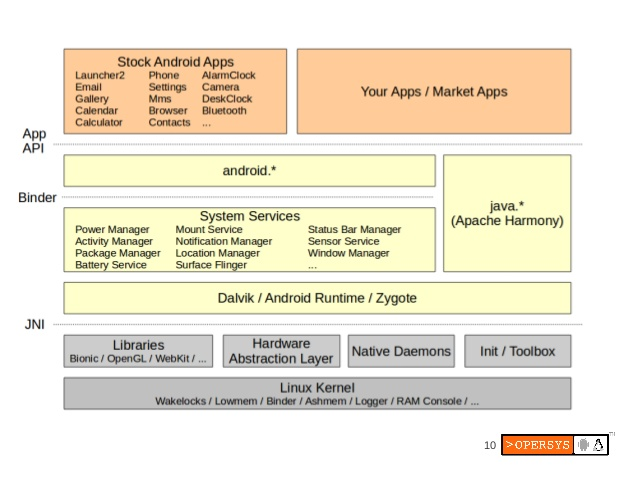
\includegraphics[width=\textwidth]{android_stack}
\centering
\caption{Android platform architecture\cite{android_stack}} 
\label{fig:android_stack}
\end{figure}

At the top of the software stack are the Android applications. Application developers use the Android API to build applications that the end user interacts with. Applications found on a device are either system apps which come installed with the stock OS or user apps which can be installed from the Google Play Store or other sources.
The Android Framework provides application developers a rich API to access the devices capabilities. The framework allows developers to manage UI interaction, access to media storage, access to device peripherals such as the baseband controller, camera, GPS, wifi controllers, inter process communication, etc.
The Android Framework and Android applications are developed in Java. Applications are compiled into Dalvik Executables (or dex files) which are then interpreted by the DalvikVM. The DalvikVM is a register based virtual machine that executes applications written for Android. The DalvikVM forms an integral part of the Android Runtime and provides a layer of abstraction to the underlying operating system. Android 4.4 (KitKat) introduced a new runtime called Android Run Time (ART) as an experimental alternative. Unlike Dalvik which used Just-In-Time compilers to convert dex bytecode into native code, ART uses Ahead-Of-Time compilers to compile the application into native code upon their installation. In Android 5.0 ART replaced Dalvik as the sole Android runtime.
In addition to the Android Framework, developers can access system services (eg. dhcpd, wpa\_supplicant,etc) and system libraries(eg bionic libc, WebKit, OpenSSL, etc) via user-space native code components. These components allow access to services and libraries that talk directly to the Linux kernel and avoid the overhead of the Android Runtime. Low-level native code operations are employed when application performance is paramount.
The final component of the Android stack is the Linux kernel. The kernel has been modified to operate smartphone hardware. Kernel drivers control device peripherals, network components, process management and file system access. Some of the android specific kernel drivers are wakelocks for power management, ashmem for anonymous shared memory, alarms, paranoid networking and Binder. Paranoid networking and Binder are important from a security perspective as the former restricts access to network sockets to applications based on their permission set and the latter implements Inter Process Communication (IPC) and an associated security mechanism. 

\FloatBarrier
\subsubsection{Application structure and components:}
Android applications are distributed in via APK (Android PacKage) files. An apk is a zip archive of several files and folders. An android application package has a folder structure as shown in Fig. \ref{fig_apk_struct}
\begin{figure}[h]
	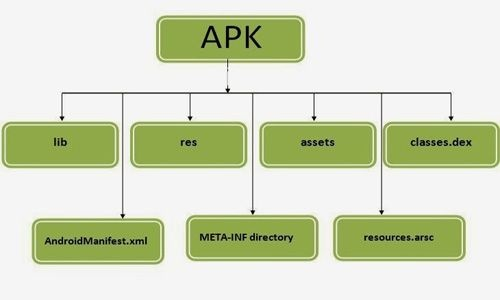
\includegraphics[width=\textwidth]{apk_structure}
	\centering
	\caption{Android package structure\cite{apk_structure}} 
	\label{fig_apk_struct}
\end{figure}
\begin{itemize}
	\item[]{\textbf{AndroidManifest.xml:} This file includes the application meta-data such as package name, minimum and maximum supported API level, permissions requested, libraries used and application components such as Activities, Services, Broadcast Receivers and Content Providers.}
	\item[]{\textbf{classes.dex:} This file contains the Dalvik bytecode to be executed by the DalvikVM.}
	\item[]{\textbf{META-INF:} This folder contains the application certificate and a list of files included in the apk along with their SHA-1 hashes.}
	\item[]{\textbf{lib:} This folder contains native binaries that the application uses. These binaries are stored in sub-folders, created for each supported CPU architecture.}
	\item[]{\textbf{assets:} This folder contians application assets that can be retrieved by the AssetManager class.}
	\item[]{\textbf{res:} This folder contains resources that are not compiled into the resources.arsc file. These include icons, images, UI layouts, menus, etc.}
	\item[]{\textbf{resources.arsc:} This file contains resources that are pre-compiled, for example application strings.}
\end{itemize}

\FloatBarrier

Having discussed the package structure we now look at the top level components of an android application. App components are entry points for the system to access the application. There are four different components with a distinct lifecycle\cite{android-fundamentals}.
\begin{itemize}
\item[]{\textbf{Activities:} These components make up the user interface of the application. An application can have more than one Activity and these are all listed in the AndroidManifest.xml file. Activities are also capable of returning results to its caller.}
\item[]{\textbf{Services:} Services are similar to Unix daemons performing background tasks without the need for user interaction. Services usually performing long-running operations or operations for remote processes. For example playing audio in the background or downloading data over the internet.} 
\item[]{\textbf{Broadcast Receivers:} These components listen to events generated by the Android Operating system or application broadcast  events. Examples of system generated broadcast events are BOOT\_COMPLETED, SMS\_RECIEVED, etc.} 
\item[]{\textbf{Content Providers:} These components provide an interface to allow sharing of stored data with other applications. Data stored on the file system, Cloud, databases etc can be queried via Content Providers. An example the Android system provides a Content Provider to access the users contacts.}
\end{itemize} 

Activities, Services and Broadcast Receivers are activated via asynchronous messages called Intents. Intents request a particular action from a component and may specify the URI of data to act on. Content Providers are not activated via Intents, rather they are activated when targeted by a request.

\subsubsection{Security model:}
This section just summarises the most significant aspects of the android security model\cite{Drake:2014:AHH:2614422} \cite{Elenkov:2014:ASI:2631372}\cite{Tyrone:2015:MAHH}.
\paragraph{\textbf{Permission model}}
Android uses two distinct but co-operating permission models as part of its security model. These two models are enforced by the Linux kernel and the other by the Android Runtime and Framework. The Linux kernel uses users and groups to enforce permissions on the file system and other android resources. This permission model commonly refereed to as the Android Sandbox, defines a set of permissions an application can request from the Android Runtime and Framework. These permissions requested by an app are listed in the AndroidManifest.xml file and are first displayed to the user when the application is installed. 

\paragraph{\textbf{Android Sandbox}}
Like traditional Linux platform Android uses user ID (UID) and Group ID (GID) paradigm, however it does not have a \textit{passwd} or \textit{group} files. It was reasoned that there would be only one user to the system (i.e. the owner of the smartphone) and so the UIDs were assigned to individual applications known as Android IDs (AID), instead of to each user on the system. Certain AIDs are reserved for privileged and system-critical applications such as those belonging to the system/user group. Like in Linux each process has its own memory space and cannot interfere with another running process. In addition to process isolation the Android Sandbox also achieves data isolation by assigning a each application a dedicated data directory with read and write permissions.

\paragraph{\textbf{Android Permissions}}
In order to allow access to hardware, system services, data storage, Internet connectivity etc., Android grants additional access rights by way of \textit{API Permissions}. Permissions requested by an application are listed in the AndroidManifest.xml file. These permissions are granted to the application at the time of installation and once granted cannot be revoked. Some API permissions map to low-level kernel permissions for example the API permission \textit{android.permission.INTERNET} which grants the application access to the Internet maps to the kernel managed group \textit{inet} which grants users the ability to open sockets. Felt et. al. developed \textit{Stowaway} to detect over-privileged Android applications \cite{felt2011android}. 

\paragraph{\textbf{Protection Levels}}
Each API permission has an associated \textit{protection level}. Some permissions are more sensitive than others and protection levels define the conditions under which the applications are granted permissions. The table below summarises the four protection levels defined by Android.
\begin{center} 
	\begin{tabular}{|cp{0.5\textwidth}|cp{0.5\textwidth}|}      
		\hline 
		Protection Level & Description \\
		\hline 
		normal & This is the default protection level and generally associated with permissions that have a low risk to the system and other applications  \\
		\hline
		dangerous &  Permissions that could allow access to sensitive data or access the devices hardware, have a protection level set as dangerous. \\
		\hline
		signature & Permissions with this protection level are only granted to applications that have been signed by the same key as the application that declared the permission. \\
		\hline
		signatureOrSystem &  Permissions with this protection level are granted to applications that have either the same signing key or are part of the system image.\\

		\hline %a line at the bottom
	\end{tabular}
\end{center} 

\paragraph{\textbf{Code signing}}
Android mandates that every application be signed before it can be installed on the system. Signing is done with digital certificates whose private key is held by the authors of the application. Code signing establishes an identity of the author of the application and provides a degree of trust with other aspects of the security framework.\\
Digital certificates can be self-signed and need not be issued by a Certificate Authority (CA) as the system does not verify certificates. Certificates are used by the Android system to perform comparisons with other applications claimed to be developed by the same author and when accepting updates for an application. This prevents forged updates and applications from being granted the same permissions associated with that certificate.

\subsubsection{Current malware landscape:}
The earliest documented Android malware were FakePlayer and DroidSMS, discovered in August 2010. Since then several researchers have surveyed android malware and its evolution \cite{felt2011survey}\cite{zhou2012dissecting}\cite{farukiandroid}\cite{le2013analysis}\cite{android_malware_analysis}. Zhou et. al \cite{zhou2012dissecting} created the Android Malware Genome project\cite{android_malware_genome} in an effort to characterize existing malware in order to aid the research community.

We provide a brief chronology of the most significant malware families from 2010 to 2015 Q1\cite{current_android_malware} describing its capabilities and mode of distribution.
\paragraph{\textbf{2010}}
	\begin{itemize}
		\item[]{\textit{FakePlayer}: This was the first malware to be discovered that targeted Android. This application masquerades as a media player and sends SMSs to premium-rate numbers without the user's knowledge \cite{jamie:FakePlayer}.}
		\item[]{\textit{FakeInst}: This application presents itself as an installer for other popular apps. When executed it sends SMSs to premium-rate numbers. \cite{joe:FakeInst}}
		\item[]{\textit{TapSnake}: This app was the Android version of the popular 1970s game of Snake. While the user played the game it would covertly send GPS co-ordinates to an attacker controlled server \cite{symantec:TapSnake}.}
		\item[]{\textit{Geinimi}: This piece of malware was first discovered in repackaged versions of legitimate apps. This trojan is capable of siphoning user data to remote servers, installing and uninstalling software, changing its list of Command \& Control servers and leaking GPS co-ordinates. It is also the first Android malware with botnet-like capabilities \cite{wyatt:Geinimi}.}
	\end{itemize}
\paragraph{\textbf{2011}}
	\begin{itemize}
		\item[]{\textit{HongTouTou/ADRD}: Another repackaged application malware that was used to increase a sites rating via fraudulent clicks. The malware would be triggered after two minutes have passed since the OS started/booted or there is a change in network connectivity or if the call state on the device changes.\cite{antiy:adrd}} 
		\item[]{\textit{DroidDream/RootCager}: This was the first malware known to use root exploits to infect a device. It uses the exploid \cite{krahmer:exploid} and rageagainstthecage\cite{krahmer:rageagainstthecage}  to break out of the Android sandbox and compromise the kernel. This allowed the malware to infect a large number of devices \cite{strazzere:droid_dream}.}
		\item[]{\textit{BaseBridge}: This trojan would attempt to exploit the udev Netlink Message Validation Local Privilege Escalation Vulnerability \cite{securityfocus:netlink} to gain root privileges. Having elevated its privileges it would install its payload which was an app to SMS premium rate numbers.}
		\item[]{\textit{DroidKungFu1}: This was another SMS trojan targeting Chinese speakers. It packaged two encrypted root exploits namely rageagainstthecage and exploid. On executing the app the exploits would be decrypted and executed to gain root privileges. On gaining root it would harvest device information and send it to a hardcoded remote server\cite{jiang:DroidKungFu}.}
		\item[]{\textit{DroidKungFu2}: Unlike its predecessor whose implementation was in Java, DroidKungFu2 was implemented in native code. Instead of sending data to a single C\&C server, it could now send the data to three servers\cite{jiang:DroidKungFu2}.}
		\item[]{\textit{DroidKungFu3}: This version of DroidKungFu was designed to be more resistant to malware detection tools at that time. It obfuscated the C\&C server URLs, encrypted its native binaries and masqueraded as a legitimate Google update\cite{jiang:DroidKungFu3}. }				
		\item[]{\textit{GoldDream:} This malware would spy on SMS messages received by users as well as incomming and outgoing calls. This data is then uploaded to remote C\&C server without the users knowing\cite{jiang:GoldDream}.}
		\item[]{\textit{Zitmo and Spitmo}: Zitmo and Spitmo were Android trojans for their Windows counterparts Zeus and SpyEye malware respectively. These malware would masquerade a banking apps and steal one-time passcodes sent from banks to the mobile phone. This data would then be sent to a remote C\&C server where the passcodes would be used to login to the victims bank account \cite{strazzere:zitmo}\cite{spreitzenbarth:spitmo}.}
		\item[]{\textit{GingerMaster}: This was the first malware to use a root exploit against Android 2.3 Gingerbread. The exploit was known as GingerBreak and is packaged as gbfm.png file. The extension is just to trick users that it is a Portable Network Graphics file. Once the device had been rooted it would remount the system partition as writeable, and install several other utilities to increase its capabilities and make removal harder \cite{jiang:Gingermaster}.}
		\item[]{\textit{AnserverBot}: This malware was consider the most sophisticated when it was first discovered. It used deep code obfuscation and dynamic code loading to make reverse engineering harder. It would install a bot client disguised as a upgrade that would run silently in the background independent of the host. This was a persistence mechanism to ensure its survival if the host was uninstalled\cite{jiang:anserverbot}.}
	\end{itemize}
\paragraph{\textbf{2012}}
	\begin{itemize}
		\item[]{\textit{NotCompatible}: This piece of malware was automatically downloaded when a user visited the malicious website from the phones browser. Once installed it would create a network proxy, which could then be used to gain access to other protected information or systems\cite{alcatel:notcompatible}.}
		\item[]{\textit{LuckyCat}: This was the first Advanced Persistent Threat (APT) to target Android. It was developed as part of a campaign to target aerospace and energy industries in Japan and Tibetan activists \cite{trendmicro:luckycat}.}
		\item[]{\textit{DrSheep}: The Android equivalent of the desktop malware tool Firesheep. It was capable of hijacking social network accounts such as Twitter, Facebook, and LinkedIn via a WIFI connection.}
	\end{itemize}
\paragraph{\textbf{2013}}
	\begin{itemize}
		\item[]{\textit{FakeDefender}: This was the first ransomeware discovered for Android. It would masquerade as Android Defender and once installed it would restrict access to any application, disable telephony services, change system settings, remove any and all applications, disable all user input buttons including Back and Home, launch itself on reboot, and execute a factory reset. Unlike typical ransomeware however it did not encrypt the data.}
		\item[]{\textit{Obad}: This is a multifunctional trojan capable of sending SMS messages to premium rate numbers, installing other malware, propagation via Bluetooth and shell execution with root privileges. Obad used multiple analysis evasion methods and exploited the Android OS to extend its administrative privileges. This made static and dynamic analysis of the malware harder and the extended privilege once granted made it impossible to remove the malware \cite{ashraf:obad}\cite{comodo:obad}.}
		\item[]{\textit{BadNews}: This malware masqueraded as an ad network which was actually a front to distribute malicious code. Thirty two apps across four different developer accounts on Google Play were discovered with this malware. The network would push code to the app once it was installed on a device. It has the ability to send fake news messages, prompt users to install applications and sends sensitive information such as the phone number and device ID to its C\&C server\cite{lookout:badnews}.}
	\end{itemize}
\paragraph{\textbf{2014}}
	\begin{itemize}
		\item[]{\textit{Torec}: This was the first trojan sample to use a .onion domain as its C\&C server. Torec was a variant of the Orbot Tor client. Using the Tor network to mask its C\&C server makes it impossible to shutdown \cite{Unuchek:torec}.}
		\item[]{\textit{OldBoot}: The first bootkit for Android, this malware had the capability to persist even after uninstallation. It partially installed itself in the boot partition and modified initialization scripts responsible for OS component installation. This allowed it to execute everytime the device was powered on \cite{jiang:oldboot}.}
		\item[]{\textit{DroidPack}: This was the first Windows malware to infect Android devices. Its payloads were DroidPack and Android Debug Bridge (ADB). The malware used ADB to connect to devices and installed the DroidPack trojan. This trojan would then uninstall legitimate banking applications and install repackaged versions of the uninstalled apps. The repackaged apps would then harvest banking credentials which would be sent to a remote C\&C server\cite{symantec:droidpack}.} 
		\item[]{\textit{DeathRing and MouaBad}: These malware samples were discovered pre-installed on smartphones popular in Asian and African countries. Instead of distributing malware via third party app markets, the attacker target the device manufactures supply chain\cite{lookout:deathring}\cite{lookout:mouabad}.}
		\item[]{\textit{CoinKrypt}: This malware turns an infected device into a crypto-currency miner for the malware. authors\cite{lookout:coinkrypt}.}
	\end{itemize}
\paragraph{\textbf{2015}}
\begin{itemize}
	\item[]{\textit{Gunpoder}: This malware family was recently discovered capable of sensitive data exfiltration, propagation via SMS and the ability to execute additional payloads. All antimalware solutions either classify it as benign or adware due to its evasion techniques.\cite{gunpoder_2015}.}
\end{itemize}


\subsection{iOS}
iOS is a propriety operating system developed and maintained by Apple Inc. for iPhones, iPads and iPod Touch devices. The first commercially released version of iOS was for the iPhone in 2007. It was then extended to support iPod Touch, iPad in 2010 and iPad mini in 2012. The first release of iOS formerly known as iPhone OS was a derivation of OS X and shares its base with the Darwin\cite{Darwin}. iPhone OS was developed by the Macintosh team at Apple lead by Scott Forstall. It was initially intended to allow developers to build web applications to run as native iPhone apps. In 2008 Apple released the first native Software Development Kit for iPhone OS. In 2010 iPhone was rebranded as iOS, which at the time of writing held the second largest share of the smartphone market.   

\subsubsection{Ecosystem:}
The iOS ecosystem consists of iOS devices manufactured by Apple, the operating system itself and iOS application developers. Unlike Google's Android, iOS is not licensed to third party hardware manufactures. The manufacturing of some components that go into the iPhone, iPad and iPod Touch are outsourced to third party manufactures but the final product is assembled at Apple factories.

The table below lists the various releases of iOS and the corresponding iPhone and iPad model that it was released with.
\begin{center} 
	\begin{tabular}{|l|c|c|c|c|}
		\hline 
		iOS/iPhone version & Release Date & iPhone model & iPad model & iPad mini\\
		\hline\hline 
		1.x & March 2008 &  1st & N/A & N/A\\
		2.x & July 2008 &  3G & N/A  & N/A \\
		3.x & June 2009 &  3GS & 1st generation & N/A \\
		4.x & June 2010 &  4 & 2 & N/A \\
		5.x & June 2011 &  4S & 3rd generation & N/A \\
		6.x & September 2012 & 5 & 4th generation & 1st generation \\
		7.x & September 2013 & 5S \& 5C & Air & 2nd generation\\
		8.x & September 2014 & 6 \& 6S & Air 2 & 3rd generation \\
		\hline %a line at the bottom
	\end{tabular}
\end{center}

\subsubsection{Software Stack:}
The iOS architecture consists of five layers, iOS applications, the Cocoa Touch layer, the Media layer, the Core Services and the Core OS layer (iOS kernel) Fig.\ref{ios_software_stack}. At the very top is the application layer the system and third party apps. iOS apps can be classified into three types. Native apps that use the publicly accessible Objective-C Framework, Web based applications that typically run within Safari, which is the default web browser, or a hybrid app which uses a combination of native and web app features. iOS applications are written in Objective-C and linked to the iOS SDK and Cocoa Touch framework.\\
The Cocoa Touch layer defines the User Interface of the application. Cocoa Touch is a collection of related frameworks which enable key technologies such as multitasking, touch-based input, push notifications, sharing content and documents, gesture recognition etc. Below the Cocoa Touch layer lies the Media layer. This layer provides services that use audio, video and graphics libraries. This framework provides support to many industry-standard audio and video formats.\\
The Core Services layer controls the Objective-C runtime and fundamental system services and applications. Some of the services this layer provides are accounts and telephony basaed services, multipeer conectivity services, iCloud storage, Data protection and File Sharing support. At the bottom of the software stack is the Core OS layer which is the iOS kernel. iOS uses the XNU kernel which is also used in Mac OS X. This layer creates an abstraction to the underlying hardware. Apps don't directly access this layer however the frameworks used by the app interact with this layer\cite{ios_layers}.
\begin{figure}[h] 
	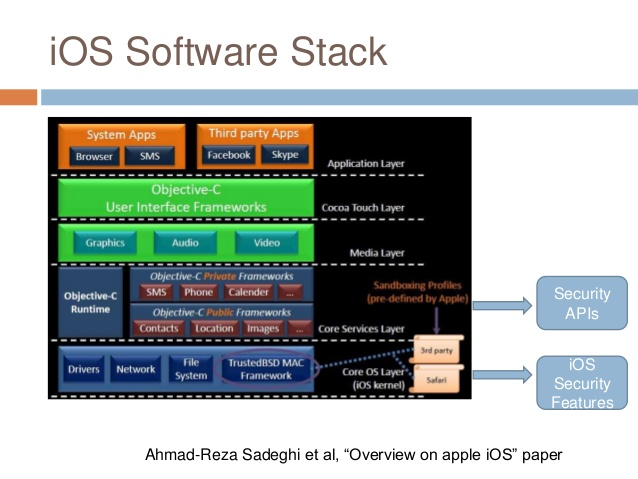
\includegraphics[width=\textwidth]{iOS_stack}
	\centering
	\caption{iOS Software Stack\cite{ios_stack}} 
	\label{ios_software_stack}
\end{figure}

\FloatBarrier
\subsubsection{Application structure and components:}
iOS applications are distributed via IPA files which are basically archives that have the .ipa extension. Uncompressing the archive reveals the following folder structure Fig. \ref{fig_ipa_structure}.
The Payload folder contains the iOS application bundle which is a folder with the applications name and suffixed with the .app extension, in this example its AppName.app.\\
AppName.app contains application binary, static resource files and additional application metadata. The iTunesArtwork file is a Portable Network Graphics (PNG) file that is used as the apps icon in iTunes and the App Store.\\
The iTunesMetadata.plist contians application meta-data such as developers name, bundle identifier and copyright information \cite{Tyrone:2015:MAHH}.
\begin{figure}[h] 
	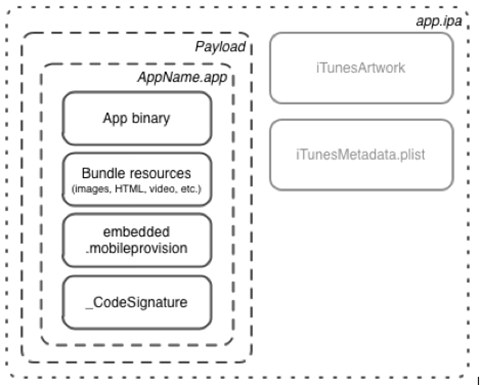
\includegraphics[width=\textwidth]{ipa_structure}
	\centering
	\caption{iOS Software Stack\cite{ipa_structure}} 
	\label{fig_ipa_structure}
\end{figure}
\FloatBarrier
 
\subsubsection{Security model:}
iOS has been designed with security at its core. The hardware and software are designed to work in tandem to provide maximum security without compromising on user experience. Apple has published a document detailing the iOS security internals\cite{apple_ios_security_internals} and its salient features are summarised below.
\paragraph{\textbf{Security Architecture}}
Security in iOS is built into the hardware and software stack. Fig. \ref{fig_ios_security_arch} shows us various components that make up the security architecture.\\
\begin{itemize}
	\item[]{Secure Boot: Each component of the boot chain is cryptographically signed by Apple to ensure its integrity. If any component of the boot process fails the chain of trust verification, the boot process is aborted and the device enters DFU (Device Firmware Upgrade) mode. The device must then be restored to factory default settings by connecting to iTunes.\\
	At the start of the boot process, the processor executes code from read-only Boot ROM. The Boot ROM is an immutable section of code that contains the Apple Root CA public key. The Boot ROM along with the public key is laid down during the chip fabrication process and is trusted implicitly. The Low-Level Bootloader (LLB) is the next component in the boot chain to be loaded once its signature has been verified by the Boot ROM. Once the LLB has finished executing it verifies and loads the next-stage bootloader, iBoot which in turn verifies and loads the iOS kernel.\\
	The secure boot chain ensures the integrity of low level components to prevent tampering and allows iOS to run only on validated Apple devices.}
	\item[]{System Software Authorization: This is a process used by iOS to upgrade the device with software updates and security patches. This process also prevents devices from being downgraded to older version so as to exploit a vulnerability in an unpatched version.\\
	System Software Authorization is done either via iTunes where a full copy of iOS is downloaded and installed, or over the air (OTA) updates where only affected components are downloaded and installed. During the upgrade the device connects to the Apple installation authorization server and sends it a list of cryptographic measurements for each component being upgraded, a random nounce for prevent replay attacks and the device's unique ID (ECID). The authorization server validates the list of measurements to check if upgrades are permitted. It then adds the ECID to the measurement and signs the result. Signed upgrades are then sent to the device from the server.\\
	The boot time chain-of-trust evaluation verifies that the signature comes from Apple and that the measurements of the items loaded from the disk, combined with the ECID match what was sent by the server.}
	\item[]{Secure Enclave: The Apple A7 and later A-series processors have a coprocessor fabricated in called the Secure Enclave. The coprocessor has its own secure boot process and personalized software upgrade process. It provides all cryptographic operations for Data Protection key management and maintains the integrity of Data Protection even if the kernel is compromised.
	It uses encrypted memory and has a built in random number generator. Communication with the application processor is achieved via an isolated interrupt-driven mailbox and shared memeory data buffers. Each Secure Enclave chip is provisioned with its own UID (unique ID) during fabrication and is inaccessible to other parts of the system. On system boot up an ephemeral key is created, entangled with its UID and used to encrypt the Secure Enclave's portion of memory space. Also the data saved to the file system by Secure Enclave is encrypted with a key entangled with the UID and an anti-replay counter.}
	\item[]{Touch ID: This is the fingerprint sensing technology that makes secure access faster and easier. Touch ID although not a replacement for passcodes overcomes the inconvenience of having to frequently enter long passcodes to unlock the device.
	Touch ID is a form of user authentication that can also be used to approve purchases from the iTunes Store, the App Store and the iBoot Store.}
\end{itemize}
\begin{figure}[h]
	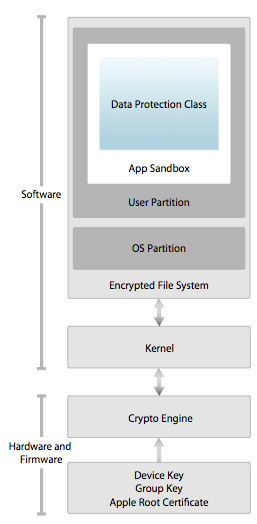
\includegraphics{ios_security_arch}
	\centering
	\caption{iOS security architecture diagram\cite{apple_ios_security_internals}} 
	\label{fig_ios_security_arch}
\end{figure}
\FloatBarrier
\paragraph{\textbf{Encryption and Data protection}}
Even if the underlying security infrastructure is compromised, iOS has additional encryption and data protection features to safeguard user data. These features are summarised below
\begin{itemize}
	\item[]{Hardware security features: Every iOS devices has a dedicated AES 256 crypto engine built into the the DMA path between the flash storage and main system memory. The device's unique ID (UID) and a device group ID (GID) are AES 256bit keys fused or compiled into the application processor and Secure Enclave during fabrication. These keys are inaccessible by either software or hardware and only the output of encryption or decryption operations is readable.\\
	UIDs are unique each iOS device and are not recorded by Apple or its suppliers. GIDs are common to all processors in a class of devices. UIDs bind data cryptographically to a device, so if memory chips are mounted on another device the files will still be inaccessible. Besides the UID and GID,
	all other cryptographic keys are created by the systems Random Number generator built into the hardware. Entropy is generated from timing variations during boot and from interrupt timing once the device has booted.\\
	Secure erasing of stored keys is equally important as creating them and iOS devices use a feature called Effaceable Storage for secure data erasure. This directly accesses and erase a small number of blocks at the hardware level using the underlying storage technology.}
	\item[]{File Data Protection: iOS uses a feature called Data Protection to protect data stored in flash memory. On creating a file on the data partition, Data Protection creates a new 256bit key for this file and uses the hardware AES engine to encrypt the file as it is written to flash memory. The per-file key is wrapped with one of several class keys, depending on the circumstances under which the file should be accessible. This wrapped per-file key is stored in the file's metadata.\\
	On opening the file the metadata is decrypted with the file system key to retrieve the wrapped per-file key. The per-file key is unwrapped with the class key which gives us the 256bit per-file key. This is then given to the AES engine which decrypts the file as it is read from memory Fig. \ref{fig_ios_file_data_protection}.\\
	The File System key is generated when iOS is first installed or when the device is wiped by a user. The File System key is not intended to provide confidentiality but is designed to provide a means of quickly erasing data. Erasing the file system key renders all files cryptographically inaccessible.}
\begin{figure}[h] 
	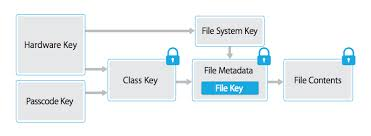
\includegraphics{file_data_protection}
	\centering
	\caption{File Data protection architecture\cite{apple_ios_security_internals}} 
	\label{fig_ios_file_data_protection}
\end{figure}
\FloatBarrier
	\item[]{Passcodes: iOS supports four-digit passcodes and arbitary length alphanumeric passcodes. In addition	to unlocking the device, a passcode provides entropy for certain encryption keys. Certain Data protection classes require a passcode to access data, thus providing security to devices under under the attackers possession.}
	\item[]{Data Protection Classes: These are policies enforced by iOS to determine when data is accessible. There are four main classes described in the table below
	\begin{center} 
		\begin{tabular}{|cp{0.5\textwidth}|cp{0.5\textwidth}|}      
			\hline
			Data Protection Class & Description \\
			\hline \hline 
			Complete \\(NSFileProtectionComplete) & The class key is protected with a key derived from the user passcode and the device UID. Once the device is locked the decrypted class key is discarded, rendering all data in this class inaccessibel until the device is unlocked with the passcode or via Touch ID  \\
			\hline
			Protected Unless Open \\ (NSFileProtectionCompleteUnlessOpen) &  Files that need to be written while the device is locked use this class. An example is a file downloading in the background. \\
			\hline
			Protected Until First User Authentication \\ (NSFileProtectionCompleteUnitlFirstUserAuthentication) & This class behaves in the same way as Complete Protection, except that the decrypted class key is not removed from memory when the device is locked. This is the default class for all third-party app data not otherwise assigned to a Data Protection class. \\
			\hline
			NoProtection \\ (NSFileProtectionNone) &  This class key is protected only with the UID, and is
			kept in Effaceable Storage. Since all the keys needed to decrypt files in this class are
			stored on the device, the encryption only affords the benefit of fast remote wipe.\\
			
			\hline %a line at the bottom
		\end{tabular}
	\end{center} 
		
	}
	\item[]{Keychain data protection: iOS keychain provides a sure container to store sensitive data such as credentials, login tokens, certificates etc. The keychain is implemented as a single SQLite database which is stored on the file system. the securityd daemon determines which keychain items each process or app can access.\\
	Keychain data is protected using a class structure similar to the one used in file Data Protection. This is summarised in the table below \cite{Tyrone:2015:MAHH}.
	\begin{center} 
		\begin{tabular}{|cp{0.5\textwidth}|cp{0.5\textwidth}|}      
			\hline
			Keychain Protection Class & Description \\
			\hline \hline
			kSecAttrAccessibleAlways & The keychain item is always accessible.  \\
			\hline
			kSecAttrAccessibleWhenUnlocked & The keychain item is accessible only when the device is unlocked. \\
			\hline
			kSecAttrAccessibleAfterFirstUnlock & The keychain item is only accessible after the first unlock from boot. \\
			\hline
			kSecAttrAccessibleAlwaysThisDeviceOnly & The keychain item is always accessible but cannot be migrated to other devices.\\
			\hline
			kSecAttrAccessibleWhenUnlockedThisDeviceOnly & The keychain item is only accessible when the device is unlocked and may not be migrated to other devices.\\
			\hline
			kSecAttrAccessibleAfterFirstUnlockThisDeviceOnly & The keychain item is accessible after the first unlock from boot and may not be migrated to other devices.\\
			\hline
			kSecAttrAccessibleWhenPasscodeSetThisDeviceOnly & Only allows you to store keychain items if a passcode is set on the device.
			These items are accessible only when a passcode is set; if the password is later unset, they cannot be decrypted.\\
			\hline %a line at the bottom
		\end{tabular}
	\end{center}
	}
	\item[]{Keybags: The keys for both file and keychain Data Protection classes are collected and managed in keybags. iOS uses the following four keybags: system, backup, escrow, and iCloud Backup.
	\begin{center} 
		\begin{tabular}{|cp{0.5\textwidth}|cp{0.5\textwidth}|}      
			\hline
			Keybag & Description \\
			\hline \hline
			System keybag & The class keys used in normal operation of the device are stored. For example, when a passcode is entered, the NSFileProtectionComplete key is loaded from the system keybag and unwrapped.  \\
			\hline
			Backup keybag & Created when an encrypted backup is made by iTunes and stored on
			the computer to which the device is backed up. A new keybag is created with a new
			set of keys, and the backed-up data is re-encrypted to these new keys. \\
			\hline
			Escrow keybag & This keybag allows iTunes to back
			up and sync without requiring the user to enter a passcode, and it allows an MDM server to remotely clear a user’s passcode. It is stored on the computer that’s used to sync with iTunes, or on the MDM server that manages the device. \\
			\hline
			iCloud Backup keybag & Similar to the backup keybag, all the class keys in this keybag are asymmetric so iCloud backups can be performed in the background\\
			\hline %a line at the bottom
		\end{tabular}
	\end{center}	
	}
\end{itemize}
\paragraph{\textbf{App security}}
Application security is critical for any smartphone security model and iOS is no exception. iOS ensures that apps are signed and verified and are sandboxed to protect user data. The salient features of app security are summarised below.
\begin{itemize}
	\item[]{App code signing: To ensure that all apps come from a trusted source and has not been tampered with, iOS requires that all executable code be signed using an Apple-issued certificate. Apps that are part of stock iOS are signed by Apple. Mandatory code signing extends the concept of chain of trust from the OS to apps, and prevents third-party apps from loading unsigned code resources or using self-modifying code.\\
	In addition to code signing, every app submitted to the app store is vetted by Apple before being made publicly available.Unlike other mobile platforms, iOS does not allow users to install potentially malicious unsigned apps from websites, or run untrusted code. At runtime, code signature checks of all executable memory pages are made as they are loaded to ensure that an app has not been modified since it was installed or last updated.}
	\item[]{Process sandboxing:All third-party apps are “sandboxed,” so they are restricted from accessing files stored by other apps or from making changes to the device. This prevents apps from gathering or modifying information stored by other apps. Each app has a unique home directory	for its files, which is randomly assigned when the app is installed. If a third-party app	needs to access information other than its own, it does so only by using services explicitly provided by iOS.\\
	System files and resources are also shielded from the user’s apps. The majority of iOS runs as the non-privileged user “mobile,” as do all third-party apps. The entire OS partition is mounted as read-only. Unnecessary tools, such as remote login services, aren’t included in the system software, and APIs do not allow apps to escalate their own privileges to modify other apps or iOS itself.}
	\item[]{Exploit Mitigations: Address space layout randomization (ASLR) protects against the exploitation of	memory corruption bugs. Built-in apps use ASLR to ensure that all memory regions are randomized upon launch. Randomly arranging the memory addresses of executable	code, system libraries, and related programming constructs reduces the likelihood of many sophisticated exploits.\\
	Further protection is provided by iOS using ARM’s Execute Never (XN) feature, which marks memory pages as non-executable. Memory pages marked as both writable and executable can be used only by apps under tightly controlled conditions: The kernel checks for the presence of the Apple-only dynamic code-signing entitlement}
\end{itemize}

\subsubsection{Current malware landscape:}
Although an overwhelming majority of smartphone malware targets Android. There have been a few malware families targeting iOS \cite{current_ios_malware}\cite{ios_malware_exists}. As iOS imporves its market share we predict an increase in malware families targeting iOS.
\paragraph{\textbf{2009}}
	\begin{itemize}
		\item[]{\textit{Trapsms}: This malware family intercepts SMS messages from the infected iOS device and forwards them to a remote server. This affects Jailbroken devices.}
		\item[]{\textit{MobileSpy}:This malware is capable of spying on incoming and outgoing calls, SMS, URLs and GPS co-ordinates which are then sent to a remote server. This affects only Jailbroken devices.}
		\item[]{\textit{Ikee/Eeki}: This was the first worm developed for iOS. It exploited the fact, that many users of jailbroken devices used the default root password of the SSH daemon. The worm would propagate by scanning the network for similar vulnerable iOS devices, change the root password once it has infected the device and siphon of the users SMS database to a remote server.}
		\item[]{\textit{Toires}:This malware was a PoC to demonstrate that it is possible to gather the following sensitive data from an iOS device by using standard SDK methods. }
	\end{itemize}
\paragraph{\textbf{2010}}
	\begin{itemize}
		\item[]{\textit{LBTM}: This is AdWare that spams the users screen with ads. When the user attempts to touch the screen it tries to dial premium rated phone numbers.}
	\end{itemize}

\paragraph{\textbf{2011}}
	\begin{itemize}
		\item[]{\textit{iKeyGuard}: This malware implements a keylogger which is capable of sending keystroke data via email to the author. This affects only Jailbroken devices.}
	\end{itemize}
	
\paragraph{\textbf{2012}}
	\begin{itemize}
		\item[]{\textit{FindCall}: This malware is sends the users personal data to a remote server.}
	\end{itemize}

\paragraph{\textbf{2013}}
\begin{itemize}
	\item[]{\textit{Riskware/Killmob}: This malware is capable of stealing call logs, SMS databases and can record video and audio. This affects Jailbroken devices.}
\end{itemize}

\paragraph{\textbf{2014}}
\begin{itemize}
	\item[]{\textit{AdThief/Spad}: This malware tweaks a developer ID that’s intended to tell ad developers when their ads are either viewed or clicked and in turn, generate revenue. In the malware’s case, infected devices funnel those small payments away from the developers to the hacker. This affects Jailbroken devices.}
	\item[]{\textit{Unfold Baby Panda}:This malware listens to outgoing SSL connections. From these connections it tries to steal the device’s Apple-ID and corresponding password and sends them to a remote server. Only Jailbroken devices are affected by this malware.}
	\item[]{\textit{PawnStorm.A and PawnStorm.B}: This is an example of an APT targeting government and military officials and personnel in defence industries. This malware family is capable of reading the users SMS database, Photo gallery, GPS co-ordinates and record audio\cite{Apvrille:pawnstorm}.}
\end{itemize}

\section{Malware Analysis Process} \label{process}
In this section we look at the goals of malware analysis and what are the question that need to be answered in the analysis report. We also present our generalized approach to analysing malware on smartphones and a potential report template to document the analysis.

\subsection{Goals of Malware Analysis}
The goal of malware analysis is to allow us to answer the following questions \cite{kris:practical_malware_analysis}.
\begin{itemize}
	\item[]{\textbf{What is the purpose of the malware?}}
	\item[]{\textbf{How did it infect the system?}}
	\item[]{\textbf{Who are the attackers and what are the resources at their disposal?}}
	\item[]{\textbf{What did it steal?}}
	\item[]{\textbf{How long has it been here?}}
	\item[]{\textbf{What are the capabilities of this malware?}}
	\item[]{\textbf{How do we identify this malware in the future?}}
\end{itemize}
Malware examination is composed of simple and complex tasks. These tasks can be broadly categorized as into four stages\cite{zeltser:analysis_stages}. These four stages are illustrated in Fig. \ref{fig_malware_analysis_stages} as a pyramid. At the bottom of the pyramid we have the easier tasks such which can be done by open source or commercially available tools but offers limited insight into the malware being analysed. As we move higher up the pyramid, the analysis gets more involved requiring a lot more effort and specialized skill set.
\begin{figure}[h] 
	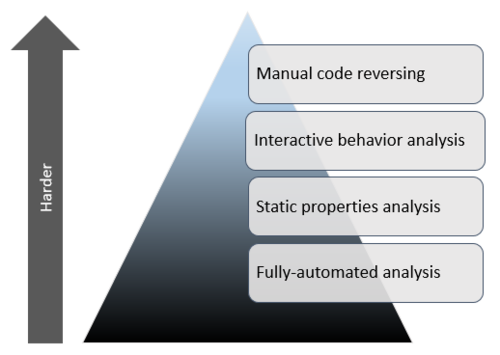
\includegraphics[width=\textwidth]{stages_of_malware_analysis}
	\centering
	\caption{Four stages of malware analysis\cite{zeltser:analysis_stages}} 
	\label{fig_malware_analysis_stages}
\end{figure}
\FloatBarrier 

The four stages can be summarised as follows
\begin{enumerate}
	\item{\textbf{Fully-automated analysis:} This is the easiest stage of malware analysis. It involves scanning the suspected sample with automated tools. These tools are designed to analyse a large number of samples and identify the ones that are potentially malicious. This saves the analyst time in having to manually analyse each sample. However these tools are not absolutely accurate and there can be cases of false-negatives and false-positives.}
	\item{\textbf{Static properties analysis:} This stage invlolves examining the sample without having to actually execute the code. This include analysing strings embedded into the file, header details, hashes, embedded resources, packer signatures, metadata such as the creation date, permissions requested, signing certificates, etc.}
	\item{\textbf{Interactive behaviour analysis:} This stage involves allowing the sample to execute within an isolated environment to observe its behaviour. This stage allows the analyst to study network communications, file operations, processes execution and utilization of system resources.}
	\item{\textbf{Manual code reversing:} This is the final stage in malware analysis and involves reverse engineering the malware sample and analysing the source code. Code analysis is time consuming and burdensome, however it reveals malware capabilities that might not be observable from behaviour analysis.}	
\end{enumerate}

\subsection{Generalized analysis approach} 
\begin{enumerate}
\item{We begin by analysing the sample with automated tools. A variety of tools exist that can be run both locally and from the web. Some malware samples are designed to evade certain automated tools, therefore it is advised to use multiple tools to analyse the sample.}
\item{The reports from the automated tools provide early indications of the samples maliciousness. However sophisticated malware have been known to use analysis evasion techniques to deceive automated tools. The analyst is therefore advised to consider other parameters in their analysis such as the origins of the sample, the frequency of the samples occurrence, etc.}
\item{The next step in the analysis process is \textit{static analysis}. We analyse the samples metadata,embedded resources, executables and other artefacts. The executables are decompiled/disassembled to retrieve the source/assembly which the analyst can then statically examine for malicious behaviour. Guidelines to static analysis are described in section \ref{gen_static_analysis_guide}.}
\item{Many samples now use several methods of obfuscation to slow down if not thwart reverse engineering. In such circumstances we first try to identify the packer being used and try to find a deobfuscator for that packer. A times the packer is not known or tools to deobfuscate the packer may not exist yet. The analyst would then have to manually unpack the executable either by hand or by building custom scripts.}
\item{Having completed our static analysis, we move towards understanding the behaviour of the sample with \textit{dynamic analysis}. The first step is to provision sandboxes for the samples targeted platform. The sample is executed within the sandbox to observe its network communication, interactions with the file-system, memory space and other device resource utilization. Guidlines to dynamic analysis are described in section \ref{gen_dynamic_analysis_guide}.}
\item{Additionally we may wish to debug the running sample within the sandbox to learn more about its behaviour that might not be immediately apparent from just black box observations. Activities such as analysis evasion techniques, persistence techniques and deobfuscation routines reveal themselves when tracing the samples execution. This information can then be used to tweak the properties of the sandbox to defeat evasion techniques.}
\item{On completion of the previous steps we generate a report to summarize the analysis and document artefacts of interest along with supporting data such as logfiles, network captures, screenshots, etc.}
\end{enumerate}

\subsection{Guidelines to creating sandboxes}
Sandbox creation and provisioning is one of the first steps in setting up a malware analysis lab. A sandbox should provide visibility, resistance to detection and scalability \cite{lastline:building_effective_sandbox}. Visibility implies that the sandbox should enable the analyst to view as much of the malware execution as possible. Secondly the sandbox must be provisioned so as to make it increasingly difficult for malware to identify its presence. Lastly it should be possible to generate multiple sandboxes so as to analyse multiple malware samples simultaneously without interference in the analysis.\\
The two options available for sandbox creation for smartphones are using physical sandboxes and emulated sandboxes. Physical sandboxes provide higher resistance to detection over emulated sandboxes but scalability is difficult. Emulated sandboxes offer greater scalability and visibility due to the flexibility they provide from its software implementation. However additional work needs to be done to make it resistant to detection. Emulators tend to provide only a subset of the underlying platform's capabilities and not complete functionality. For example emulators allow mocking phone calls but not sending and receiving actual phone calls. This makes it easy for malware to detect such sandboxes.We suggest that the analyst create both physical and emulated sandboxes to analyse malware. Additionally the sandbox should have capabilities to extract artefacts of interest such as databases, logfiles, memory dumps, etc to the analysis workstation.
 
\subsection{Guidelines to static analysis} \label{gen_static_analysis_guide}
Static analysis allows us to examine a sample without having to execute it. This section provides some guidelines on what to look for while performing static analysis.
\begin{enumerate}
	\item{Given a sample identify the file type and the platform it targets. Smartphone applications are generally archives that contain executable files and other resources. Extract and examine its contents. Look for abnormal file names and anomalies in the modified, accessed and created timestamps. This helps to some extent in identifying repackaged applications.}
	\item{Compute MD5, SHA1, SHA256 and Fuzzy hashes so as to compare them with existing malware databases or to detect a repackaged app from its original.}
	\item{Generally apps are required to be signed before they are installed on the device. Obtaining signing information from certificates included in the application bundle could help identify the authors and/or origins of the sample.}
	\item{Identify permissions requested by the application (e.g. AndroidManifest.xml found in Android applications).}
	\item{Analyze app contents for embedded strings and payloads within binaries and other resource files. Android malware authors have been known to embed payloads within resources \cite{strazzere:dex_education}}.
	\item{A major part of static analysis is decompiling the binaries to reveal the source code. When analysing the source we look for sensitive function calls, communication patterns (TCP,HTTP,SMS etc), encryption/decryption routines and keys, Encoding (e.g. Base64) and interaction with the file system. Malware authors use several tricks to make it harder if not thwart code inspection. Some methods are obfuscation, encryption and triggering exceptions in reversing tools \cite{strazzere:dex_education}. Analyst are advised to use multiple tools for code inspection and not rely on a single tool. Obfuscation and encryption may slow down the analysis and it may be prudent to attempt dynamic analysis before attempting deobfuscation.}
\end{enumerate}
\subsection{Guidelines to dynamic analysis} \label{gen_dynamic_analysis_guide}
Dynamic analysis involves executing the sample in a sandbox to observe its behaviour. The first order of business is to have a dedicated workstation solely for analysis and connected to an isolated network. This is a fail-safe measure incase the malware sample escapes the sandbox. We are not aware of known smartphone malware that is known to escape sanboxes but such sophistication could be implemented in the future. The behaviours to observe are listed as follows
\begin{enumerate}
	\item{\textbf{Network Communication:} The analysis workstation should be configured to act as a proxy from network traffic from the sandboxes. This includes both physical and emulated sandboxes. By proxying traffic to the workstation it makes it easier to setup traffic monitoring tools and other traffic injection utilities.\\
	When observing traffic patterns look for connections to unknown hosts, data being transmitted between host and sandbox and attempt to identify the communication protocol.}
	\item{\textbf{File operations:} Observing file operations such as files deployed and files being read from and written to give clues on the data being processes by the application and other operational dependencies.}
	\item{\textbf{Application tracing:} This allows the analyst to attach a debugger to the running sample to trace its execution and access to resources being used, such as file handles, network operations, memory addresses etc.}
\end{enumerate}

\subsection{Generating an analysis report}
The malware analysis report typically consists of the following sections \cite{zeltser:malwarereport} \cite{soni:malware_report}.
\begin{itemize}
	\item[]{\textbf{Executive Summary:} This section should summarise and highlight the key-points of the analysis. The reader of the report should get a gist of the specimens nature, capabilities, mode of infection and other relevant characteristics.}
	\item[]{\textbf{Identification:} This should include name, size, hashes (MD5, SHA-1 and Fuzzy hashes), packer information,  obfuscator information, known aliases if any, etc.}
	\item[]{\textbf{Capabilities:} This section should describe the capabilities of the malware such as permissions requested and used, data leakage, interaction with the attacker, analysis evasion mechanism, etc.}
	\item[]{\textbf{Dependencies:} This includes any network or file resources that the malware is dependent on for its execution, minimum and maximum version of operating system and other platform dependencies.}
	\item[]{\textbf{Behavioural and Code analysis findings:} This section documents the observations made during behavioural and code analysis. }
	\item[]{\textbf{Supporting data:} This consists of log files, screenshots, network traffic captures, function listings, string excerpts and other artefacts that support the investigation.}
	\item[]{\textbf{Incident Recommendations:} This is section provides indicators for detecting the malware on other systems.}
\end{itemize}
A template for the analysis report can be found in Appendix \ref{analysis_report_template}.

\section{Analysing Android Malware} \label{android_malware_analysis}
Of all the extant smartphone platforms Android has been the most popular target for malware. This section provides an implementation of the proposed malware analysis for Android.
\subsection{Creating an analysis lab}
This section describes the process of creating and provisioning physical and virtual sandboxes, configuring the network and setting up application tracing. The following steps serve as a guide to setting up the environment.
\begin{enumerate}
	\item{Arrange a dedicated workstation (Laptop or desktop) for the sole purpose of malware analysis. The workstation should have sufficient processing power and memory to run multiple Android emulators in parallel. Minimum system requirements are listed below
		\begin{itemize}
			\item{CPU: 2.5Ghz}
			\item{Memory: 4GB}
			\item{Harddisk space: 20GB}
			\item{Networking capabilities}
		\end{itemize}
	We recommend installing any popular flavour of Linux on the workstation since some of the tools being used come pre-packaged with most Linux distributions. However a Windows or a Mac workstation can also be used, with suitable alternatives for the tools used.
	}
	\item{Having installed Linux, ensure that the following packages are downloaded and installed on the system.
		\begin{enumerate}
			\item{\textit{Java runtime and Jdk 7 or greater}: Some of the tools used are java based and require the runtime and jdk to be installed.}
			\item{\textit{Android SDK}: This contains the build tools, platform tools and other utilities to work with the Android OS.}
			\item{\textit{Android Studio}: This is the official IDE for Android from Google. This will allow us to debug android applications.}
			\item{\textit{ssdeep}: This tool allows us to generate fuzzy hashes\cite{breitinger2012fuzzy} of samples being analysed.}
			\item{\textit{apktool}: Allows decompilation and repackaging of apk files.}
			\item{\textit{dex2jar}: Converts Dalvik bytecode to Java bytecode.}
			\item{\textit{jd}: Decompiles Java bytecode to Java source code.}
			\item{\textit{jadx}: Decompiles apks to java source code.}
			\item{\textit{Virtualbox}: Virtualization tool required to run Android Emulators via Genymotion. Version 4.3 or above is recommended.}
			\item{\textit{Wireshark}: Tool used to capture and analyze network packets.}
			\item{\textit{Burpsuite}: This tool allows us to create an HTTP proxy to intercept HTTP communication from the malware sample.}
			\item{\textit{FakeDNS}: This script allows us to spoof DNS replies.}
			\item{\textit{Genymotion}: This tool allows us to create emulated Android devices. Although Android emulators can be created using Android Virtual Device (AVD) that comes bundled with the Android Sdk. Genymotion is faster and its user friendly interface makes it easily configurable, unlike AVD emulators which require a lot more work to configure. The free version of Genymotion comes with limited features, if you have the resources we recommend purchasing a licence to the full version.}
			\item{\textit{SQLite Database Browser}: This tool allows us to view SQLite databases.} 
		\end{enumerate}
	}
	\item{Get a couple of android smartphones capable of running the last two releases of Android. The phones will need to be rooted since some of our forensic tools require root privileges. Ensure that USB debugging and installation from unknown sources is enabled. These settings can be found under Settings \textgreater Developer Options \textgreater USB Debugging and Settings \textgreater Security \textgreater Unknown sources respectively.}
	\item{The following forensic applications need to be installed on both physical and emulated  Android devices
		\begin{enumerate}
			\item{\textit{AFLogical}: This app allows us to capture Call logs, address book and SMS/MMS messages.}
			\item{\textit{tcpdump}: Not really an app. This binary allows us to capture network traffic form the device. The binary can be extracted out of known tcpdump wrappers for Android and installed to the /system/bin partition. Details of how to achieve can be found at gadgetcat.wordpress.com/2011/09/11/tcpdump-on-android/}
			\item{\textit{Titanium Backup}: This app lets you backup the entire system. We use this to restore the state of the sandboxes once we have completed our analysis.}
		\end{enumerate}	
	}
	\item{We now configure our network to proxy HTTP traffic from the sandboxes to the analysis workstation.
		\begin{enumerate}
			\item{Run Burpsuite and add a new proxy listener. Bind the new listener to the IP address of the workstation and a port number (generally 8080). Enable support for invisible proxying for this listener.}
			\item{The network adapter configuration for Genymotion emulated devices can be accessed by via Virtualbox (Fig. \ref{fig:vbox_manager}). Each emulator can be configured to use a maximum of 4 network adapters. The first adapter is reserved by Genymotion. The second adapter should be bridged with Host's adapter connected to the internet. This can be done by editing the emulators hardware configuration from Virtualbox (Fig. \ref{fig:vbox_network}).}
			\item{To proxy traffic from physical devices they should both connect to the same network. If the analysis workstation and physical device are connected to the same wireless network then modify the wireless connection on the physical device and manually specify the proxy servers IP address and port number.}
		\end{enumerate}
	}
\end{enumerate}
\begin{figure*}
	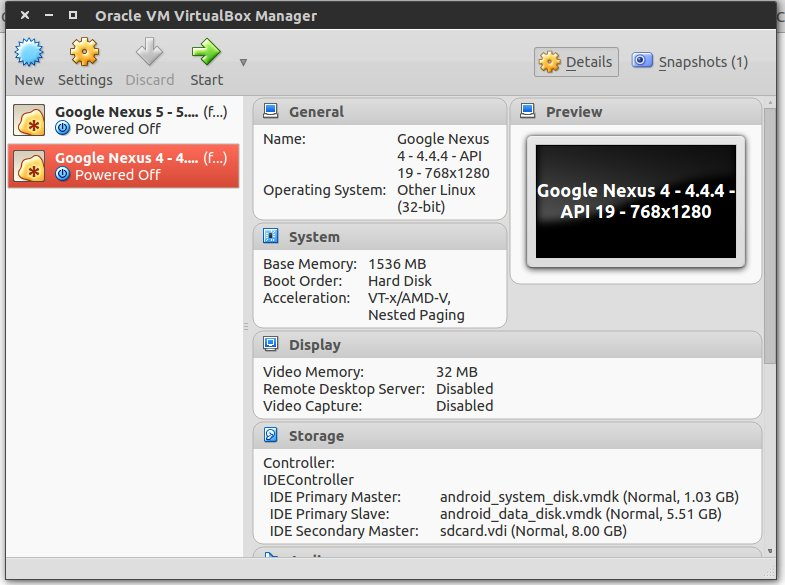
\includegraphics[width=\textwidth]{virtualbox_device_manager}
	\centering
	\caption{Virtualbox manager} 
	\label{fig:vbox_manager}
		
	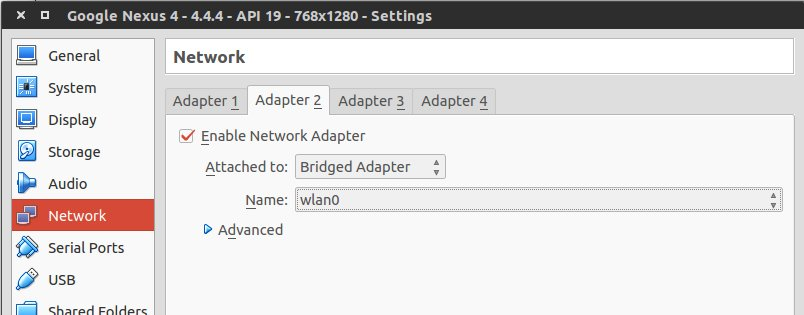
\includegraphics[width=\textwidth]{vbox_network_configuration}
	\centering
	\caption{Network Adapter configuration} 
	\label{fig:vbox_network}
\end{figure*}
\FloatBarrier
\subsection{Analysing Malware}
\begin{enumerate}
	\item{Upload the sample to some of the online analysis services mentioned below or search their hashes on the internet.
		\begin{itemize}
			\item{Virustotal (\textit{www.virustotal.com/})}
			\item{Andrubis (\textit{anubis.iseclab.org/})}
			\item{Joe Sandbox (\textit{www.apk-analyzer.net})}
			\item{Dexter (\textit{dexter.dexlabs.org/})}
			\item{CopperDroid (\textit{copperdroid.isg.rhul.ac.uk/copperdroid/})}
			\item{ForeSafe (\textit{www.foresafe.com/submit})}
			\item{Metascan (\textit{www.metascan-online.com})}
		\end{itemize}
	This would give us an indication on the maliciousness of the sample and other information regarding its capabilities and internal structure.
	}
	\item{Decompile the apk using apktool \cite{apktool} and examine its contents. 
		\begin{itemize}
			\item{Inspect the contents of the apk for suspicious files and directories. Inspect resource files for embedded payloads.}
			\item{Review AndroidManifest.xml and note the minimum and targeted Sdk version, permissions and features used and the various activites, services, boradcast receivers and content providers declared.}
			\item{Review signing certificate information found in the META-INF folder.}
		\end{itemize}
	}
	\item{Unzip the apk to extract the classes.dex file. Inspect the embedded strings within the dex file using the \textit{strings} utility found on most linux distributions for anything that might be suspicious}	
	\item{Apktool decompiles the dex file to smali code. To convert the Dalvik bytecode to java bytecode, decompile classes.dex using dex2jar\cite{dex2jar}. This generates a \textit{.jar} file which can then be reversed to java source using tools such as jd or jadx. A good point to start analysing the code would be the main Activity defined in the AndroidMainfest.xml}
	\item{From analysing the code create a hypothesis on what the sample might be doing. Based on this we develop test scenarios to trigger the samples malicious code when executed within our sandboxes. Observe the samples behaviour under the test and gather information to validate our hypothesis.}
	\item{We begin our dynamic analysis by installing the sample on to the sandboxes using the Android Debug Bridge (ADB). Note the files deployed to the filesystem when the apk is installed.}
	\item{Start network captures from either within the sandbox or on the proxy server. Utilities like tcpdump\cite{tcpdump} allow captures from multiple interfaces, ensure that the correct interface is selected or capture traffic from all interfaces.}
	\item{Once the captures are running, execute the app. Interact with the app and document its behaviour.}
	\item{Execute a test scenario, record its behaviour and extract relevant data from the sandbox.}
	\item{Repeat the previous step until all test cases have been executed.}
	\item{Application tracing can be done using Android Studio and the Dalvik Debug Monitor (DDMS).Debugging on an emulator allows access to all running processes. Application tracing on a physical device however requires that the sample be debuggable. If the sample is not debuggable we can repackage it with the debuggable option enabled. The following steps describe how to repackage the app.
	\begin{enumerate}
		\item{Decompile the app using apktool\cite{apktool} to an output folder}
		\item{Edit the AndroidManifest.xml file using a text editor and add the attribute \textit{android:debuggable=true} to the applicaiton element tag. Save the AndroidManifest.xml file.}
		\item{Rebuild the app from the output folder using apktool.}
	\end{enumerate}
	}
	\item{Having completed our analysis we document the investigation in our analysis report.}
\end{enumerate}

\subsection{Case study}
To demonstrate our process for Android malware we present a case study of a malware sample. We begin our investigation by uploading the sample to some of the online analysis services. The results of automated analysis from Virustotal and Andrubis are shown in Fig. \ref{fig:virustotal_sample_upload} and Fig. \ref{fig:andrubis_sample_upload}.
\begin{figure*}[h]
	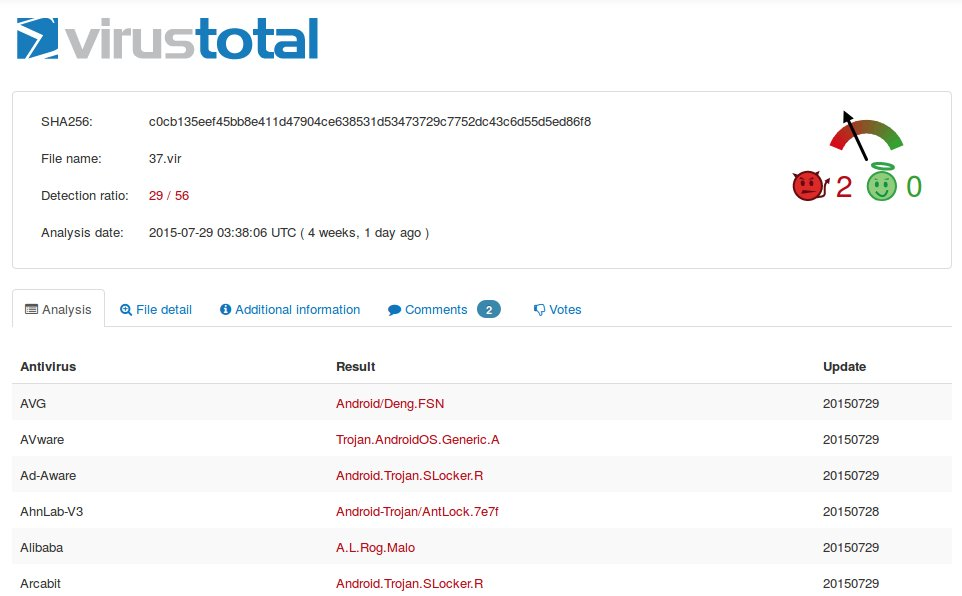
\includegraphics[width=\textwidth]{virustotal_sample_upload}
	\centering
	\caption{Sample analysis from Virustotal} 
	\label{fig:virustotal_sample_upload}
	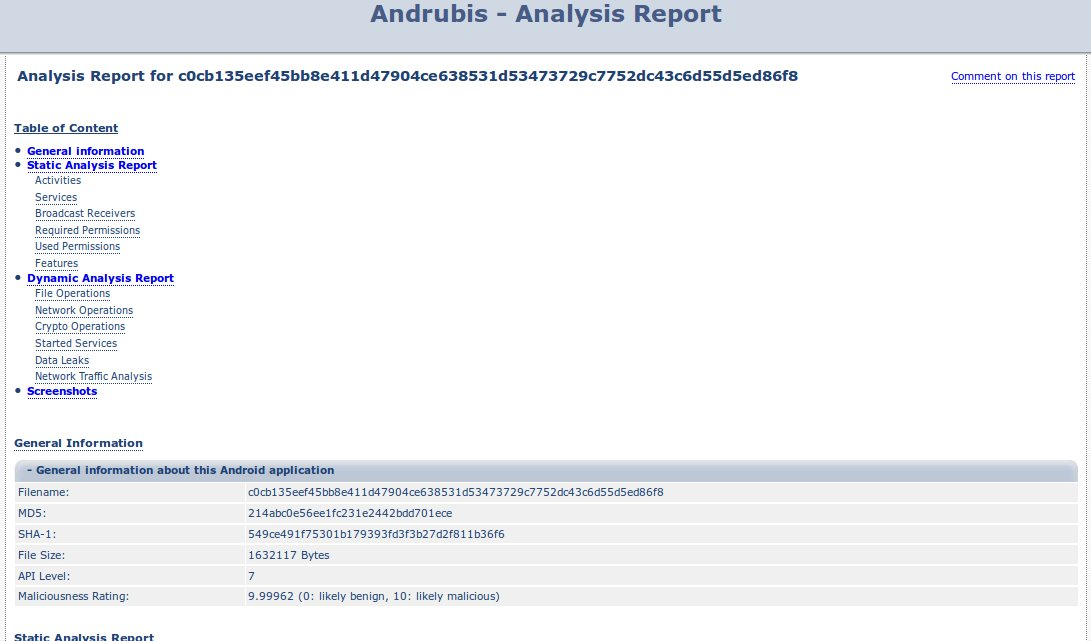
\includegraphics[width=\textwidth]{andrubis_sample_upload}
	\centering
	\caption{Sample analysis from Andrubis} 
	\label{fig:andrubis_sample_upload}
\end{figure*}
The analysis from these tools indicates that the sample is malicious. This sample has been analyzed in the past and ideally an analyst would lookup the detailed analysis reports to complete his/her investigation. For the purpose of this demonstration we assume that this hasn't been analysed before and are only aware of its maliciousness.\\
The tools also provide useful information about the internals of the malware which can be used during static analysis shown in Fig. \ref{fig:virustotal_sample_analysis} and Fig. \ref{fig:andrubis_sample_analysis}.
\begin{figure*}
	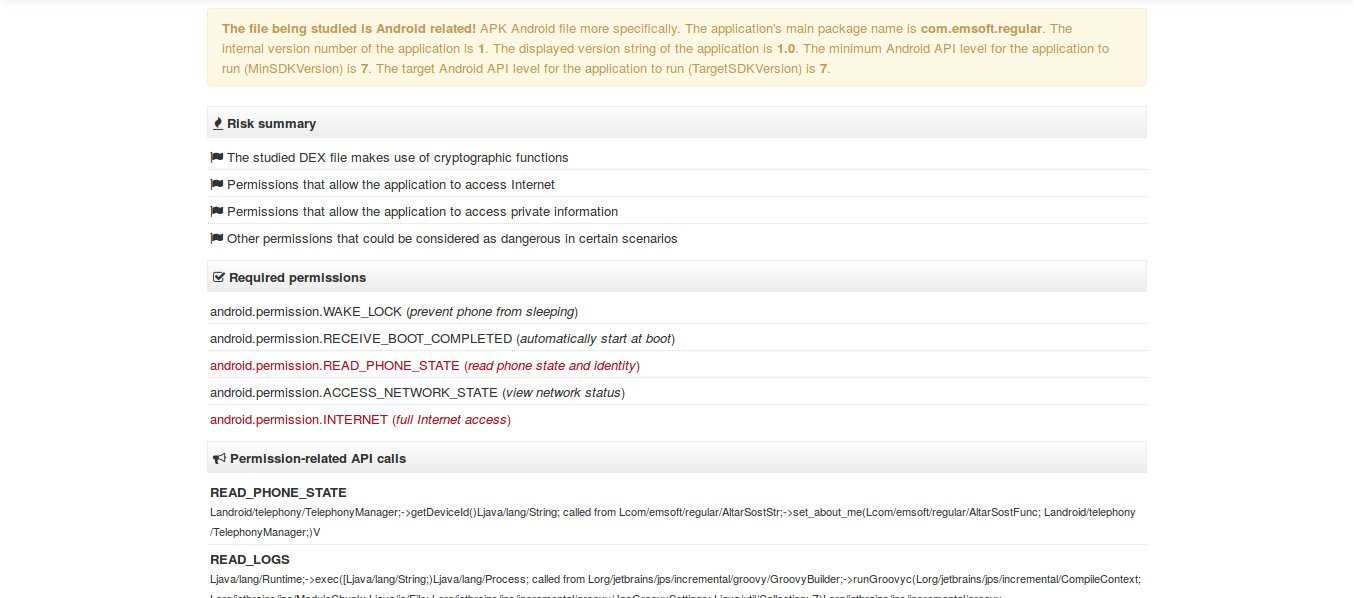
\includegraphics[width=\textwidth]{virustotal_sample_analysis}
	\centering
	\caption{Risk summary from Virustotal} 
	\label{fig:virustotal_sample_analysis}
	
	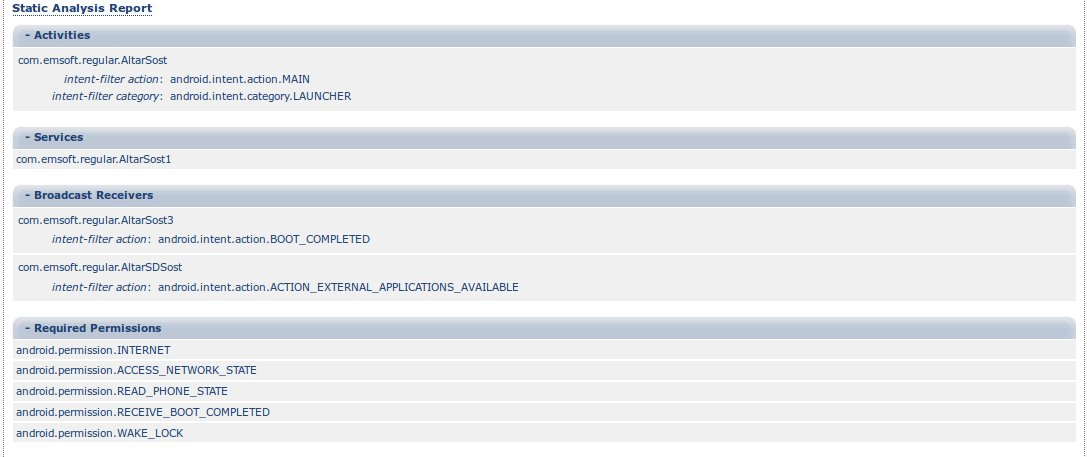
\includegraphics[width=\textwidth]{andrubis_sample_analysis}
	\centering
	\caption{Static analysis from Andrubis} 
	\label{fig:andrubis_sample_analysis}
\end{figure*} 
\FloatBarrier 
Armed with this knowledge we proceed to statically analyze the sample. We decompile the apk using apktool Fig. \ref{fig:apk_decompilation} to analyze its contents Fig. \ref{fig:apk_contents}.
\begin{figure*}
	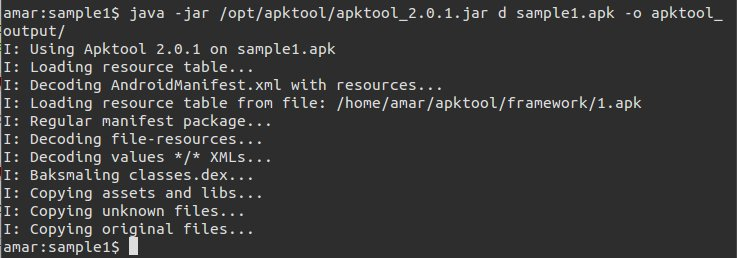
\includegraphics[width=\textwidth]{apktool_decompilation}
	\centering
	\caption{Using apktool to decompile the apk} 
	\label{fig:apk_decompilation}
	
	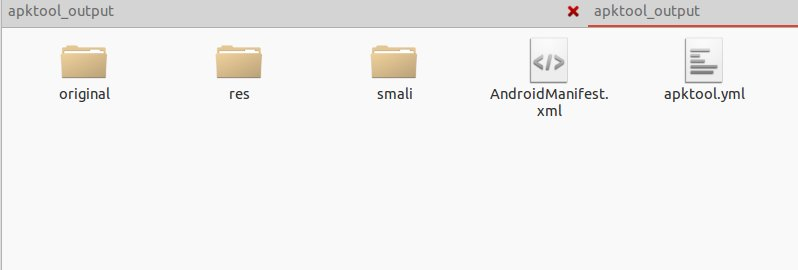
\includegraphics[width=\textwidth]{sample_contents}
	\centering
	\caption{Sample contents after decompilation} 
	\label{fig:apk_contents}
\end{figure*}
\FloatBarrier
Inspecting the AndroidManifest.xml file we learn the samples permission list and components Fig. \ref{fig:androidmanifest}. The certificate doesn't contain any interesting information nor are there any other suspicious files. 
\begin{figure}
	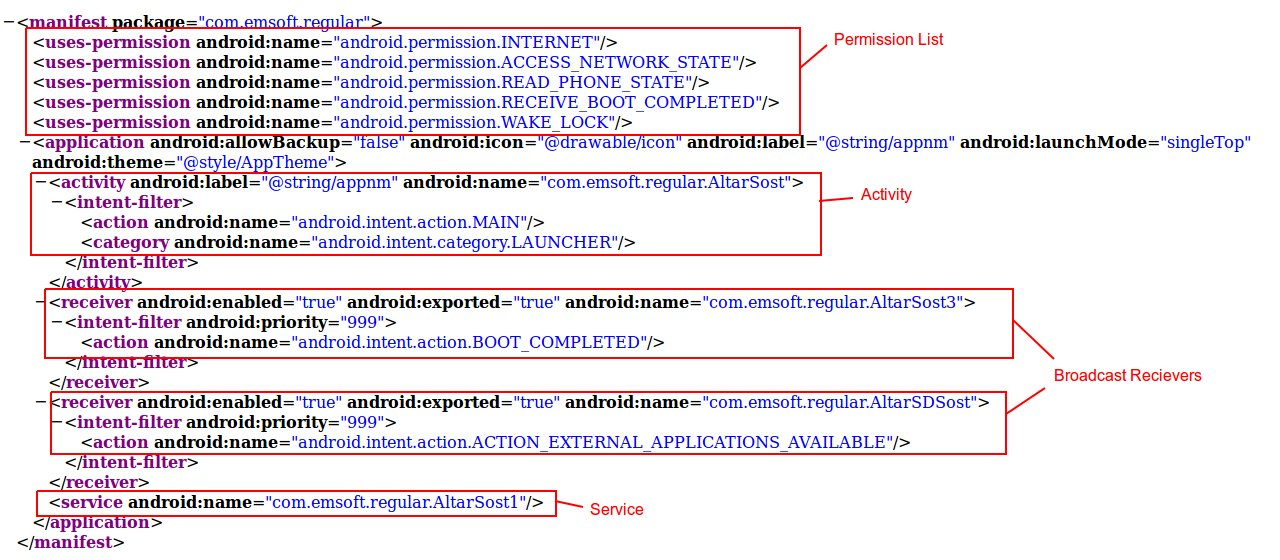
\includegraphics[width=\textwidth]{androidmanifest}
	\centering
	\caption{Examining the AndroidManifest.xml} 
	\label{fig:androidmanifest}
\end{figure} 
\FloatBarrier
We use we analyse the java source using jadx Fig. \ref{fig:jadx-gui} We being our code analysis by looking at the Main activity which was listed in AndroidManifest.xml.
\begin{figure}
	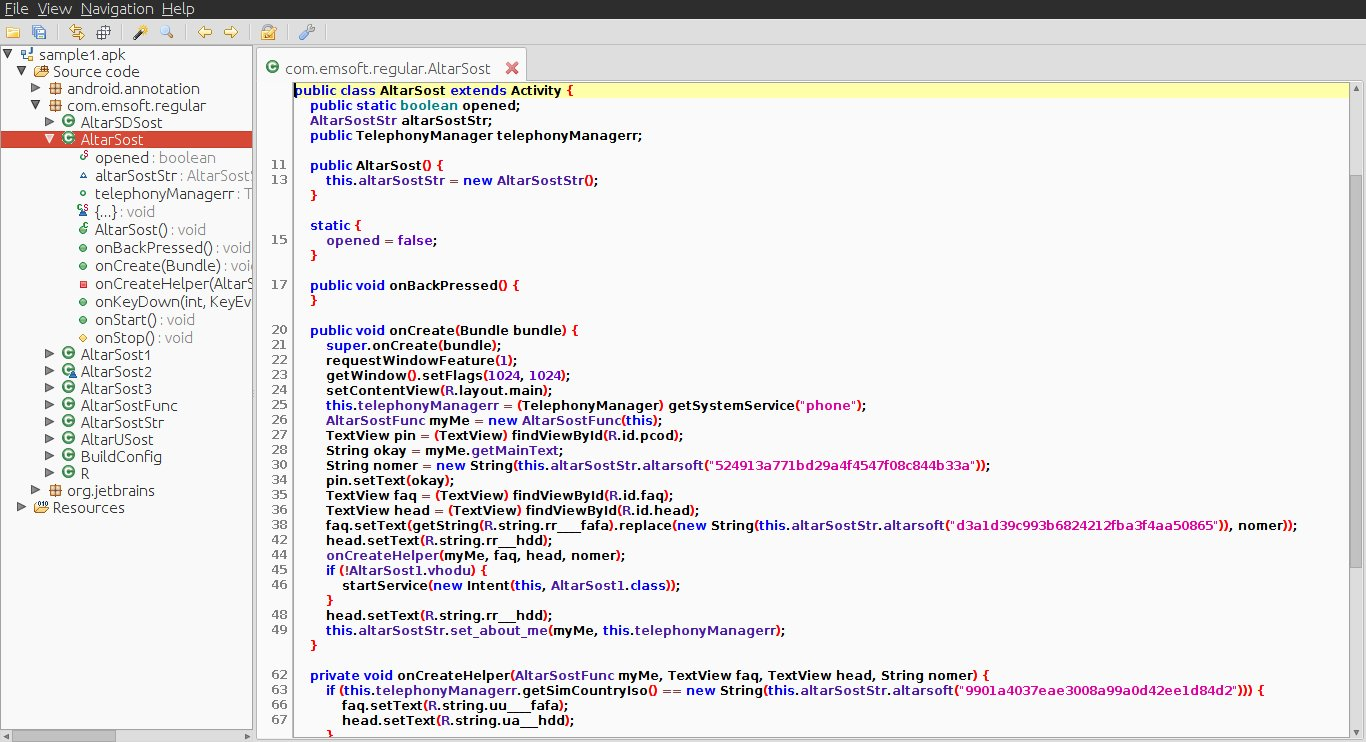
\includegraphics[width=\textwidth]{jadx-gui_analysis}
	\centering
	\caption{Code analysis with jadx-gui} 
	\label{fig:jadx-gui}
\end{figure}
\FloatBarrier 
We observe that the sample uses some form of string encryption highlighted in Fig. \ref{fig:string_encryption}.
\begin{figure}
	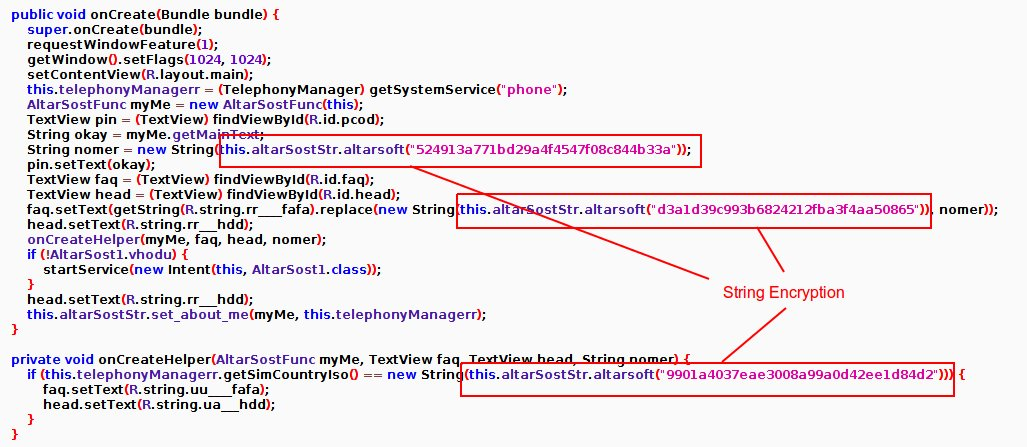
\includegraphics[width=\textwidth]{string_encryption}
	\centering
	\caption{String encryption} 
	\label{fig:string_encryption}
\end{figure}
\FloatBarrier
We find the decryption routine in the class \textbf{com.emsoft.regular.AltarSostStr}. We learn that AES (Advanced Encryption Standard) cipher in CBC (Cipher block chainging) mode is being used. The IV (initialization vector) and the key are also included in the code Fig. \ref{fig:decryption_routine}.
\begin{figure}
	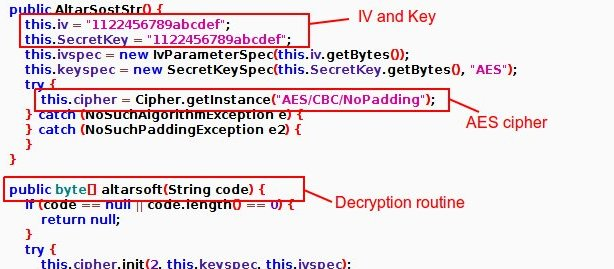
\includegraphics[width=\textwidth]{encryption_routine}
	\centering
	\caption{AES encryption/decryption routine} 
	\label{fig:decryption_routine}
\end{figure}
\FloatBarrier
Using the cipher and keying information we can decrypt the strings which reveals the following data Fig \ref{fig:decrypted_strings}.
\begin{figure}
	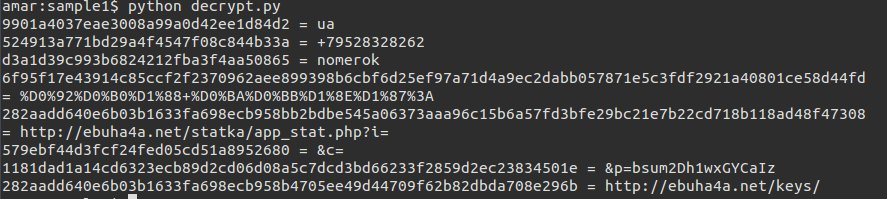
\includegraphics[width=\textwidth]{decrypted_strings}
	\centering
	\caption{Decrypted strings from the source} 
	\label{fig:decrypted_strings}
\end{figure}
\FloatBarrier
With this information we continue our code analysis and find that the sample gathers information about the device, namely the IMEI number and the SIM number (Fig. \ref{fig:information_gathering}) and then sends it off to a remote server via a HTTP GET message (Fig. \ref{fig:http_request}). The remote server is a URL that was hardcoded and encrypted in the source and is listed in Fig. \ref{fig:decrypted_strings}.
\begin{figure*}
	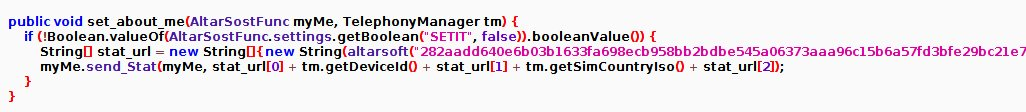
\includegraphics[width=\textwidth]{information_gathering}
	\centering
	\caption{Information gathering routine} 
	\label{fig:information_gathering}
	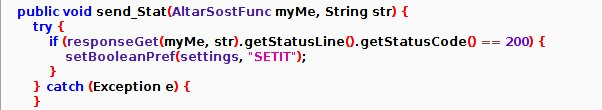
\includegraphics[width=\textwidth]{http_request}
	\centering
	\caption{HTTP request} 
	\label{fig:http_request}
\end{figure*} 
\FloatBarrier
At this point we are fairly convinced that this is a Trojan designed to steal device identification information. We continue our investigation by installing the sample in our sandbox to observe its behaviour. We use a emulated sandbox for this purpose running Android 4.4 KitKat.\\
We install the sample using the Android Debug Bridge (Fig. \ref{fig:apk_installation}) to the emulator sandbox (Fig. \ref{fig:emulator_install})
\begin{figure*}
	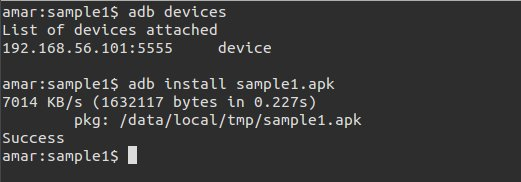
\includegraphics[width=\textwidth]{apk_install}
	\centering
	\caption{Installing the sample with adb} 
	\label{fig:apk_installation}
	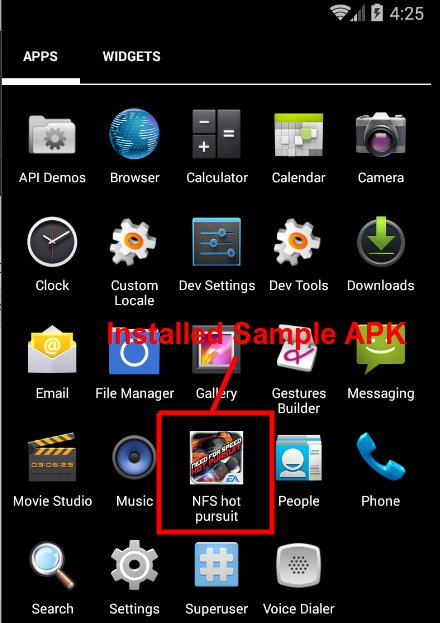
\includegraphics[width=\textwidth]{apk_installed_on_emulator}
	\centering
	\caption{Sample installed on the emulator} 
	\label{fig:emulator_install}
\end{figure*}
\FloatBarrier
The sample masquerades as a popular car racing game for android. We know that the sample uses HTTP to communicate with a remote host so our first test would be to execute the app and intercept its HTTP communication. We start the proxy listener on Burpsuite and run a network capture using ADB (Fig. \ref{fig:tcpdump_caputre}).
\begin{figure}
	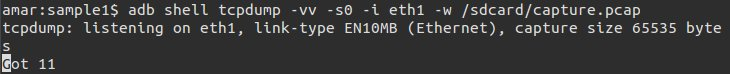
\includegraphics[width=\textwidth]{tcpdump_capture}
	\centering
	\caption{Tcpdump capture} 
	\label{fig:tcpdump_capture}
\end{figure}
\FloatBarrier
On running the app we are greeted with the following message (Fig. \ref{fig:screenshot}). Which translates to 
\begin{displayquote}
"For viewing of child porn your phone is locked !
To unlock your phone pay 500 rubles.\\ 
1. Find your nearest terminal QIWI payment system\\
2. Go to the terminal and select completion QIWI VISA WALLET\\
3. Enter your phone number +79528328262 and click Next\\ 
4. A window appears comment - then enter your key that is listed above\\
5. Put money into terminal and press pay\\
6. In the course of 180 minutes after the receipt of the payment your phone will be unlocked.\\
7. As can pay via Messenger and mobile shops Euroset\\
CAUTION: Trying to unlock the phone yourself will:
To complete lock your phone, and the loss of all important information (photos, videos, music).
Without further possibility of release and recovery."
The app would also start service that ensured the device stayed awake and would constantly display the screen. This made exiting the app difficult.
\end{displayquote}
\begin{figure}
	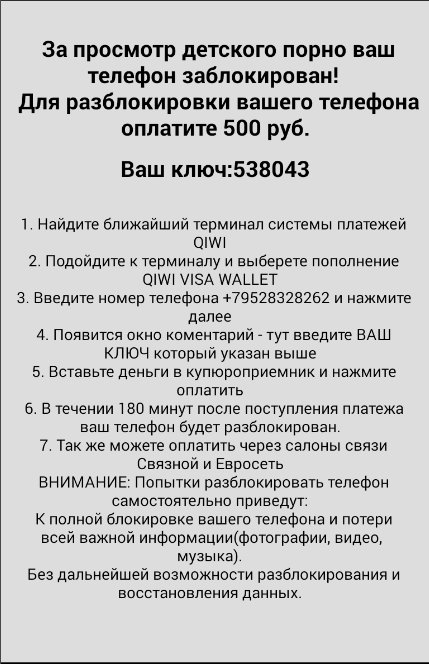
\includegraphics[width=\textwidth]{screenshot}
	\centering
	\caption{Screenshot from the sandbox} 
	\label{fig:screenshot}
\end{figure}
\FloatBarrier
The Burpsuite proxy intercepts the HTTP GET message from the sandbox (Fig. \ref{fig:burpsuite_capture}) revealing the remote host and the Device ID being siphoned off.
\begin{figure}
	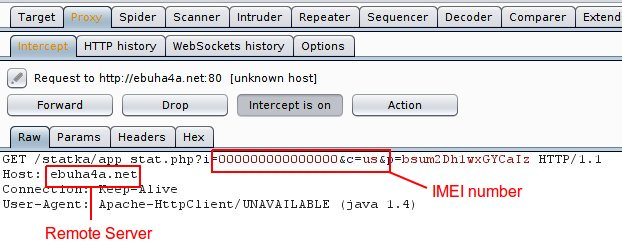
\includegraphics[width=\textwidth]{burpsuite_capture}
	\centering
	\caption{Burpsuite capture} 
	\label{fig:burpsuite_capture}
\end{figure}
\FloatBarrier
We stop the tcpdump capture and pull the capture file to the workstation (Fig. \ref{fig:tcpdump_capture_pull}). We analyse the capture file with wireshark which reveals the same information (Fig. \ref{fig:wireshark_capture}).
\begin{figure}
	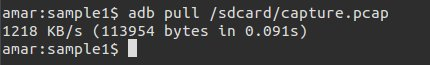
\includegraphics[width=\textwidth]{tcpdump_capture_pull}
	\centering
	\caption{Extracting the network capture to the workstation} 
	\label{fig:tcpdump_capture_pull}
\end{figure}
\begin{figure}
	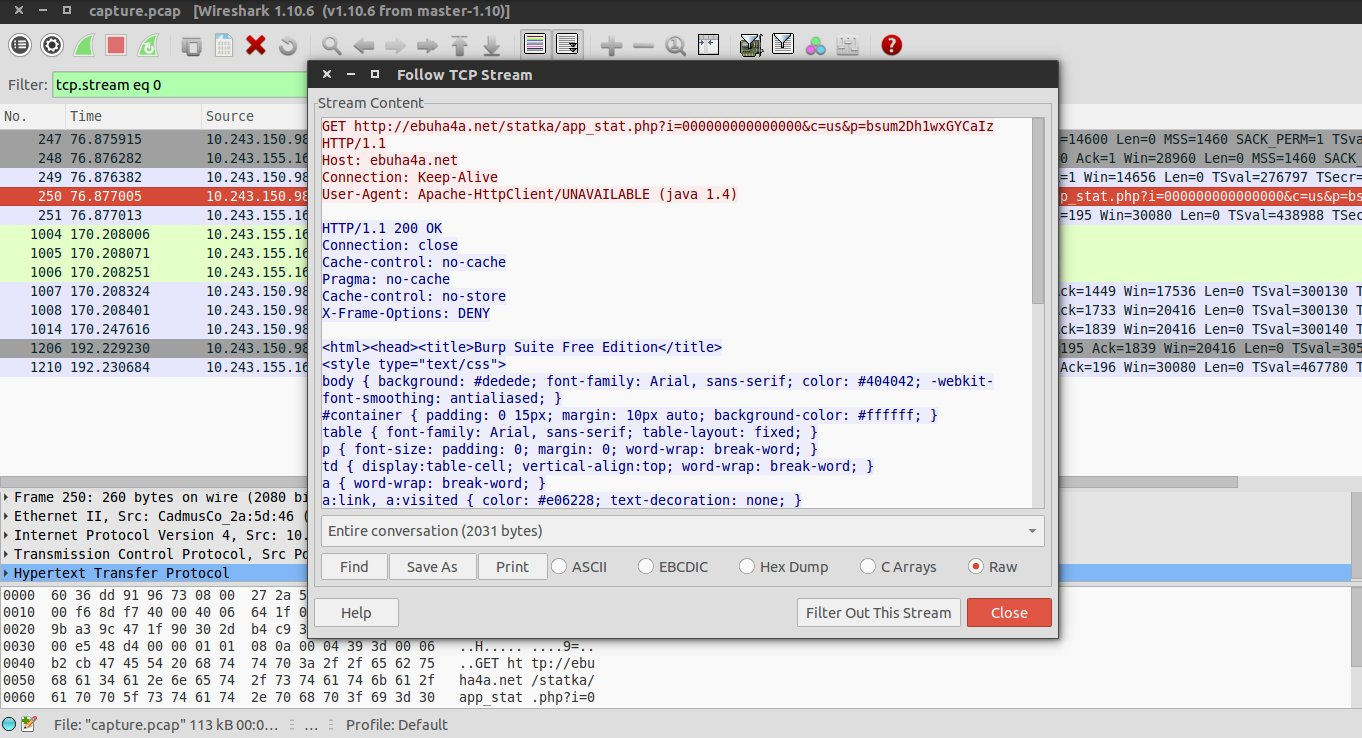
\includegraphics[width=\textwidth]{wireshark_analysis}
	\centering
	\caption{Wireshark trace} 
	\label{fig:wireshark_capture}
\end{figure}
\FloatBarrier
Thus our investigation concludes that the malware sample was a Trojan that would leak device identification information to a remote server. It used some Social Engineering to trick unsuspecting users into paying a ransom to have their devices unlocked.

\section{Limitations} \label{limitations}
We have identified two limitations to our analysis process. These are the problems of detecting colluding applications and limitations of analysis tools. We briefly discuss these problems and current research being done solve these issues.
\subsection{Detection of colluding apps}
A majority of malware analysis methodologies are designed to detect maliciousness in individual apps. Very little has been done in detecting colluding apps \cite{marforio2012analysis} \cite{bugiel2012towards}. Android permission restrictions for example can be bypassed by colluding apps whose combined permissions allow greater capabilities that neither app could individually accomplish. For example consider an app permitted to access personal data, which passes the data to a second app allowed to transmit data over the network. While collusion is not a widespread threat today, it certainly looks to be the next phase of malware evolution.

\subsection{Limitations of analysis tools}
Malware authors have been known to use various anti-analysis techniques to break tools \cite{strazzere:dex_education}. For example the Obad\cite{ashraf:obad} android malware would corrupt the conversion of its dalvik bytecode to java bytecode when by exploiting a bug in dex2jar. This has since been patched, however similar exploits could be leveraged in other analysis tools. We advise the reader to use the most up-to-date versions of their analysis tools and if possible use multiple tools to achieve the same objective.   

\section{Conclusion} \label{conculsion}
This project achieved it primary objectives of surveying the malware landscape for smartphones and creating a generalized process to analyse smartphone malware. We used this generalized analysis process to develop a specialized one for Android Malware. As part of future work we would like to develop a similar process to analyse iOS malware and even automate some parts of the process to improve efficiency.

\bibliographystyle{plain}
\bibliography{bibliography}
\appendix
\addcontentsline{toc}{chapter}{Appendices}
\addtocontents{toc}{\protect\setcounter{tocdepth}{1}}
\newpage
\section{Appendix: Analysis Report Template}
Title:\\
Investigator:\\
Date:\\

\subsection{Executive Summary}

\subsection{Identification}
\begin{enumerate}
\item{Filename}
\item{File size}
\item{File type}
\item{MAC timestamps}
\item{Hashes (md5, sha1, sha256, fuzzy)}
\item{Signing Information (Certificates)}
\item{TrID - Packer info}
\item{Aliases}
\end{enumerate}
\subsection{Capabilities}

\subsection{Dependencies}

\subsection{Static Analysis}
\begin{enumerate}
\item{Top level components}
\item{Execution points of entry}
\item{Embedded strings}
\item{Code related observations (Reflection, Obfuscation, Encryption, Native code, etc)}
\item{File contents}
\item{package contents}
\item{files created/deployed on the system}
\end{enumerate}

\subsection{Dynamic Analysis}
\begin{enumerate}
\item{Network traffic analysis}
\item{DNS Queries}
\item{HTTP Conversations}
\item{TCP/UDP communication}
\item{File operations (files read and written)}
\item{Services/Processes started}
\item{Data leaked}
\end{enumerate}

\subsection{Supporting Data}
\begin{enumerate}
\item{Log files}
\item{Network traces}
\item{Screenshots}
\item{Other data (database dumps, config files, etc)}
\end{enumerate}
\subsection{Conclusion}


\end{document}
